\chapter{Resultados}
\label{cap:Resultados}

En este capítulo se expondrán los resultados obtenidos a lo largo del desarrollo del proyecto, tras aplicar la metodología definida en el Capítulo \ref{cap:Metodologia}.

De esta manera, se detallará en primer lugar la "Estructura general" que se ha seguido para el desarrollo del proyecto con la visión general y la arquitectura del producto. A continuación, se ha incorporado un "Sprint 0" donde se especifican las necesidades y funcionalidades que se buscan desarrollar a lo largo de los sprints y que formarán la base del proyecto. Por último, se especifican en detalle todos los sprints desarrollados en este proyecto. 

\section{Estructura general}
\label{sec:EstructuraGeneral}

A continuación, es detallada la estructura general del proyecto, en la cual se muestra una visión global del producto compuesto por las necesidades que hacen necesario el desarrollo de este proyecto, el producto, el colectivo al cual va dirigido y los beneficios que se consiguen con dicho producto. Además, se muestra en detalle la arquitectura (lógica, software y funcional) del JS desarrollado en este proyecto.

\subsection{Visión Global}
\label{sec:VisionGlobal}

Como se indicó anteriormente en la sección \ref{sec:ObjetivoP}, el OP de este proyecto consiste en el diseño y desarrollo de un JS, cuyo aprovechamiento sirva para la enseñanza y el apoyo hacia aquellos usuarios que desean aprender conocimientos sobre el nuevo modelo de desarrollar software llamado DGS y en especial, conocer como se lleva a cabo la labor de gestionar proyectos de estas características, utilizando técnicas de gamificación e inteligencia artificial. En esta sección, se utiliza "The Product Vision Board"\footnote{\url{https://www.romanpichler.com/tools/product-vision-board/}} para describir, visualizar y validar la visión del producto a desarrollar, indicándose el grupo destinatario, necesidades del usuario, características clave del producto y beneficios del producto.

\subsubsection*{Grupo Objetivo}

El JS obtenido como resultado estará destinado en especial a estudiantes de ingeniería de software que desean aprender conocimientos sobre como se lleva a cabo el desarrollo de software en proyectos DGS, además de experimentar como llevar a cabo la gestión de este tipo de proyectos. Por otro lado, también estará dirigido a aquellos profesionales de la ingeniería del software que deseen ampliar sus conocimientos en otros modelos de desarrollar software, en especial con esta nueva tendencia, y así estar entrenados ante situaciones que puedan ocurrir en este tipo de proyectos y poder trabajar en un futuro en un entorno real.

\subsubsection*{Necesidades}

La aparición de este nuevo modelo de desarrollo y la importancia que está tomando en los últimos años en el mundo laboral, hace necesaria la existencia de una buena educación y enseñanza de los aspectos y conceptos que lo engloban tanto en el ámbito estudiantil como en el laboral. Incluso, se añade la manifestación del fracaso de un gran número de proyectos con entornos globales debido, en especial mediada a su desconocimiento por parte de los miembros y a la difícil gestión que conlleva esta clase de proyectos, por lo que se hace necesario un entrenamiento previo.

\subsubsection*{Producto}

Con este proyecto de TFG, se pretende obtener como resultado un JS de escritorio que permita a los jugadores jugar diferentes partidas, en donde el jugador (con el rol de jefe de proyecto) deberá gestionar un proyecto DGS ficticio, en el cual aparecerán múltiples situaciones o contratiempos que puedan ocurrir en un ambiente de estas características, las cuales deberán ser solventadas por el jugador.

\subsubsection*{Beneficios}

Los beneficios que conlleva la utilización de esta herramienta consisten en el aprendizaje de un nuevo modelo de desarrollo de software, el cual está tomando cada vez más importancia y puede ser desconocido por un gran número de personas en la actualidad. Además, permite entrenarse en un escenario virtual conociéndose así las situaciones que puedan darse en un proyecto real de estas características, y poder afrontar con éxito la gestión del mismo.

\subsection{Arquitectura}
\label{sec:Arquitectura}

A continuación, se detallará la arquitectura que se ha diseñado para conseguir el desarrollo de Global-Manager. Para ello, en este apartado se indican los componentes técnicos y funcionales de la arquitectura del juego.

\subsubsection*{Componentes técnicos}
\label{sec:ComponentesTecnicos}

En esta sección, se explicará la parte técnica que caracteriza a Global-Manager, es decir la arquitectura desarrollada para la construcción del juego. La arquitectura de la aplicación se puede desglosar en dos puntos de vista: lógico y software.

\paragraph*{Arquitectura Lógica}

La arquitectura lógica está compuesta por todos los módulos que componen el juego, en la figura \ref{fig:ArquitecturaLogica} se puede observar la arquitectura lógica del JS.

% TODO: Insertar figura con los modulos del juego.

Los módulos expuestos en el juego son los siguientes:

\begin{itemize}
	\item \textbf{Módulo cuestionario:} Se compone de un conjunto de preguntas tipo test sobre conceptos relacionados con la gestión de proyectos y DGS que deben ser conocidas por un jefe de proyectos globales. Además, se pregunta al jugador sobre sus conocimientos, estudios y experiencias relacionadas con dichos temas. Este módulo se utiliza para crear un nuevo jugador en el sistema, para ello se expone al jugador a dicho cuestionario, con el fin de calcular un nivel de jugador y evaluar así sus conocimientos, proporcionándole una experiencia de juego acorde a sus capacidades.
	\item \textbf{Módulo configuración:} Contiene un conjunto de elementos y conceptos relacionados con la configuración inicial que se debe llevar a cabo en un proyecto de DGS, ayudando al jugador a familiarizarse con dichos conceptos. Con cada configuración del proyecto que se lleva a cabo, el juego calcula automáticamente en tiempo real un conjunto de factores de éxito para proporcionar al usuario si la configuración que está llevando a cabo es correcta o no. A su vez, se calcula un nivel de dificultad del proyecto. Por otro lado, para aquellos jugadores más inexpertos en el tema, se proporciona la opción de recalcular la configuración en función de su nivel de jugador.
	\item \textbf{Módulo juego:} Provee el sistema para ejecutar la partida del juego en función de la configuración del proyecto llevada a cabo. A lo largo de la partida, el módulo proporcionará diferentes eventos que el jugador deberá gestionar y solventar con éxito. El módulo evaluará el comportamiento del jugador y decidirá si ha adquirido nuevos conocimientos o necesita mejorar algunos aspectos.
	\item \textbf{Módulo interfaz:} Proporciona el medio para la interacción del estudiante con Global-Manager, a través de una interfaz gráfica de usuario. El diseño y desarrollo de la interfaz se ha llevado a cabo según los principios del diseño, implementación y evaluación de sistemas computacionales interactivos para su utilización por seres humanos, \emph{Human Computer Interaction} (HCI). De esta manera, se busca poner en práctica los procesos para la construcción de interfaces siguiendo el criterio de usabilidad, en el caso de los videojuegos, de jugabilidad.
\end{itemize}

\paragraph*{Arquitectura Software}

La arquitectura software del JS está compuesto por un conjunto de capas en donde se dividen las componentes tecnológicas y software del juego utilizadas para su desarrollo. En la figura \ref{fig:ArquitecturaSoftware} se puede observar la arquitectura software de Global-Manager.

\begin{figure}[htb]
	\centering
	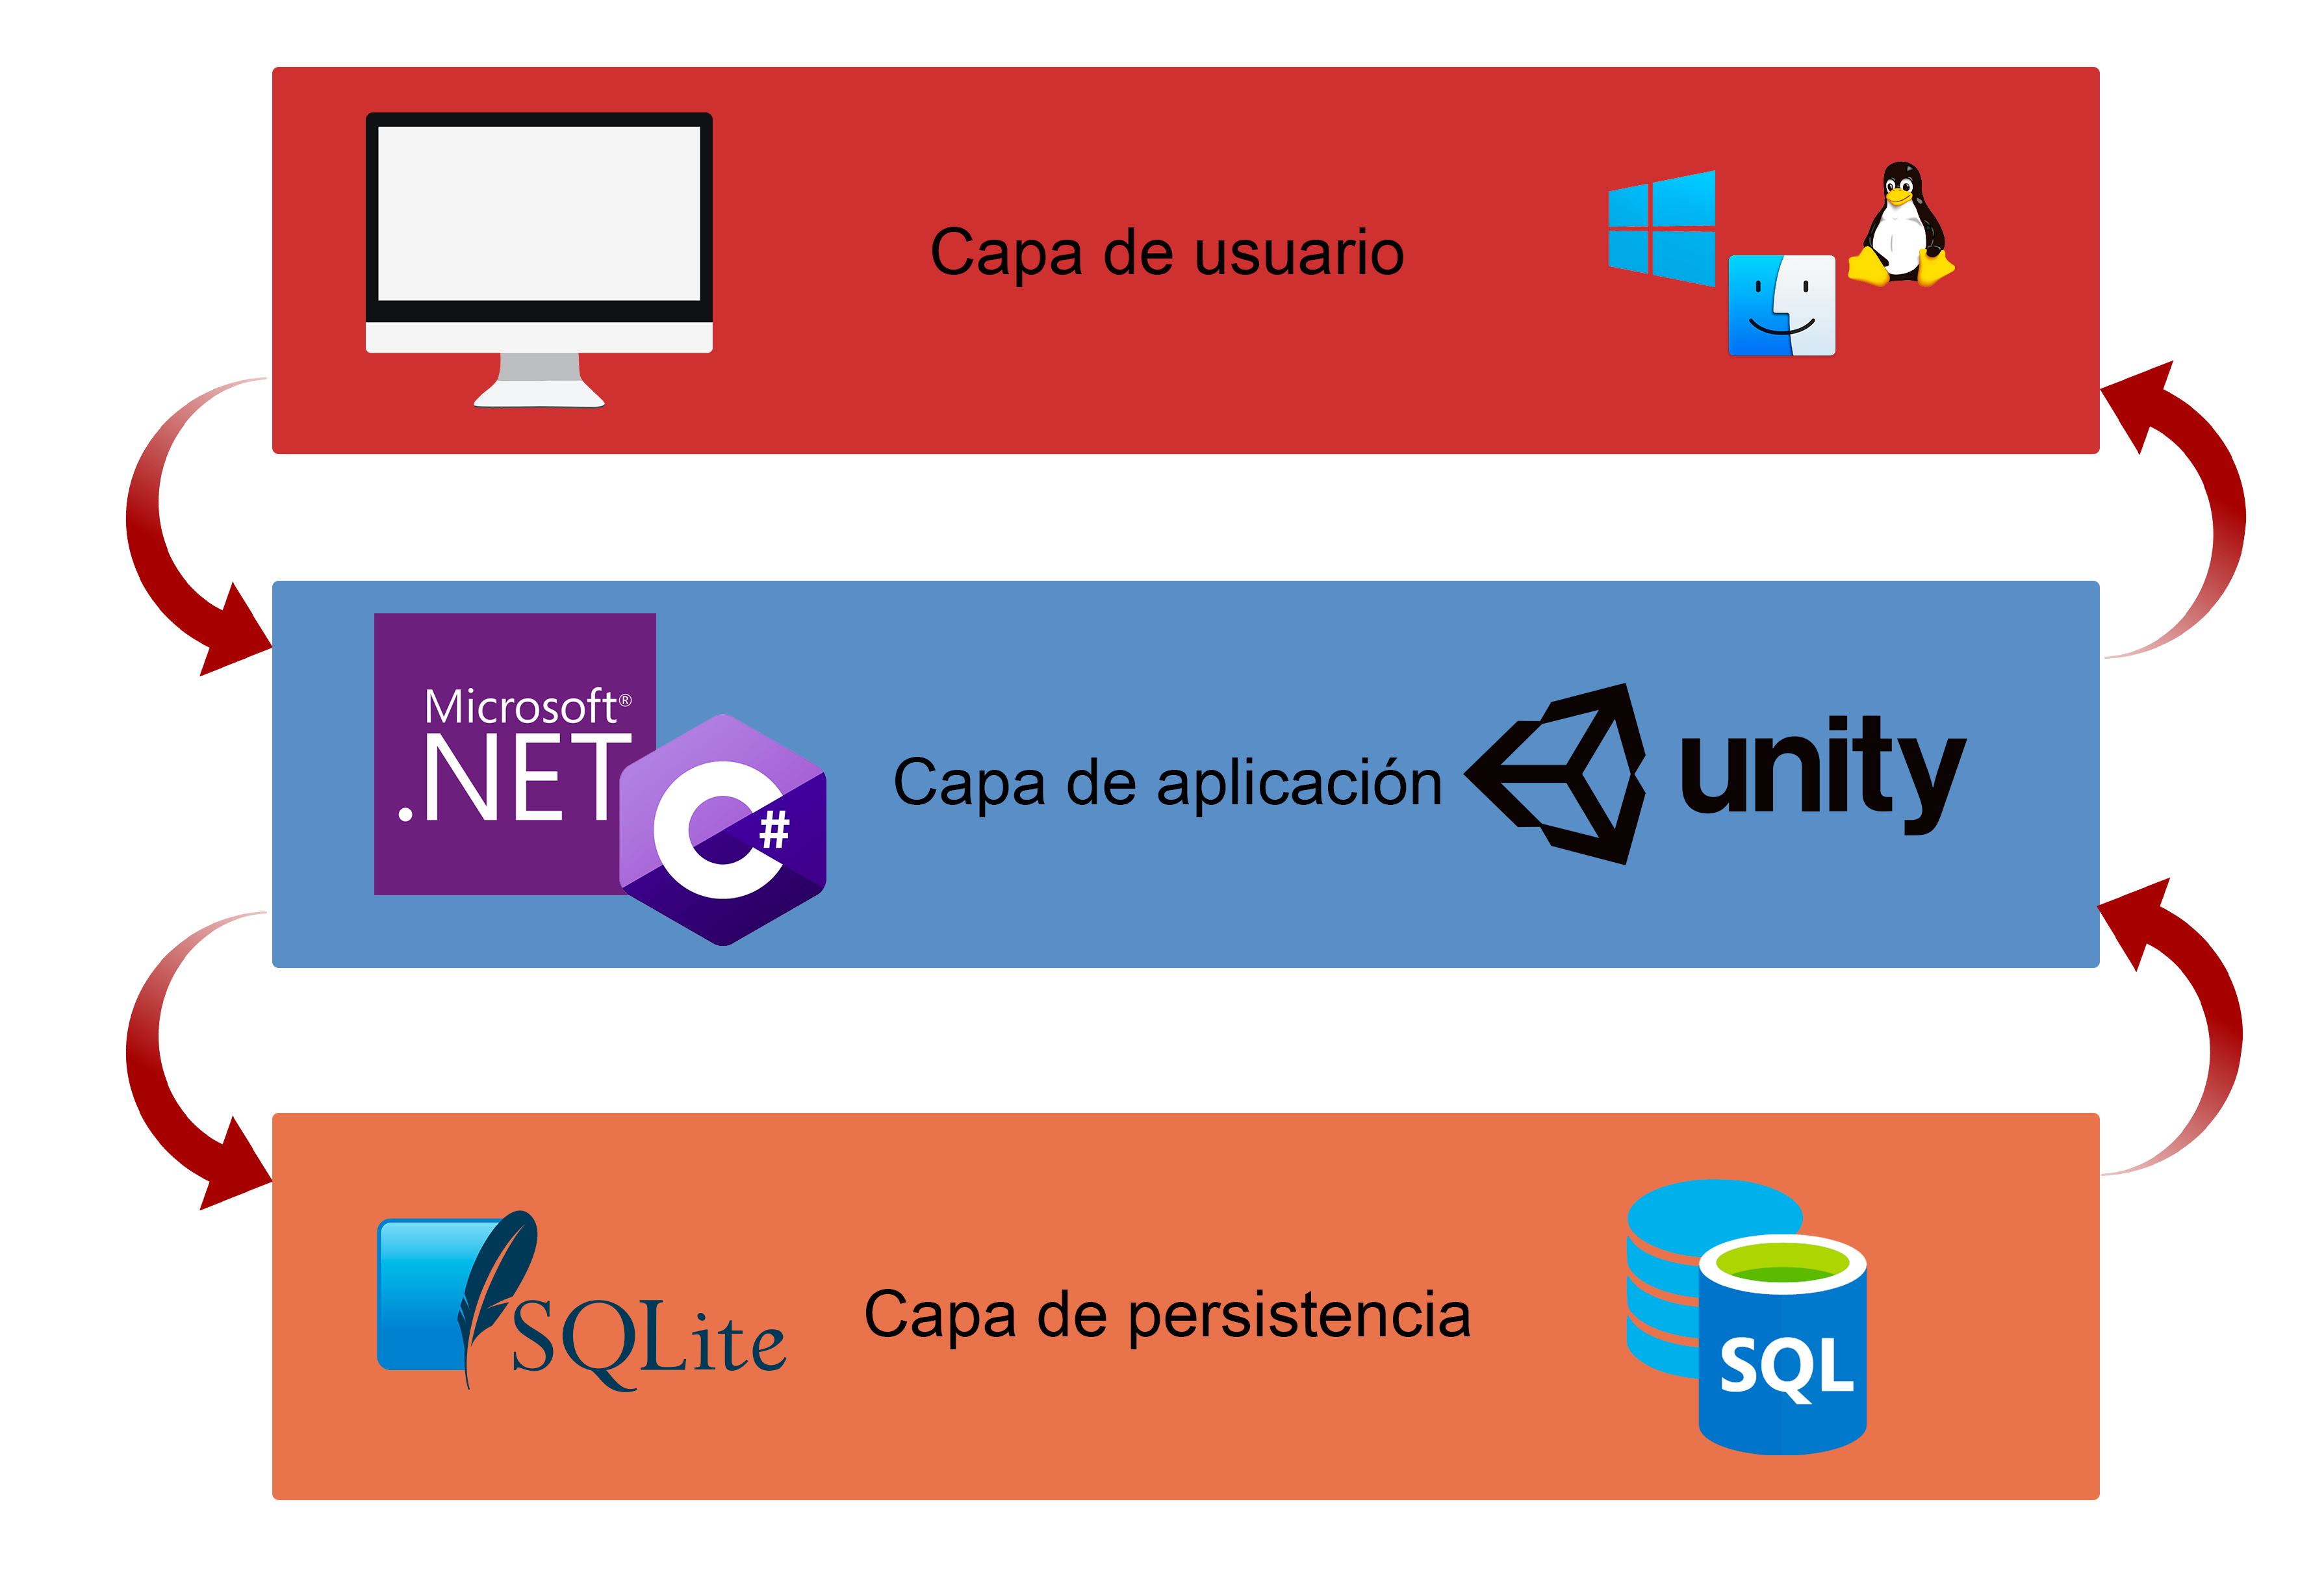
\includegraphics[width=0.95\linewidth]{ArquitecturaSoftware}
	\caption[Arquitectura software de Global-Manager]{Arquitectura software de Global-Manager}
	\label{fig:ArquitecturaSoftware}
\end{figure}

Esta arquitectura software esta compuesta por tres capas:

\begin{itemize}
	\item \textbf{Capa de usuario.} Representa el entorno sobre el cual se podrá ejecutar la aplicación. En nuestro caso, el JS consistirá en una aplicación de escritorio, la cual se podrá ejecutar en los sistemas operativos \emph{Windows}, \emph{Linux} y \emph{Mac OS}.
	\item \textbf{Capa de aplicación.} Consiste en la capa que hace referencia al JS, el cual consistirá en un proyecto \emph{.NET Framework}, en el cual se utiliza el motor de videojuegos y físicas, \emph{Unity} junto con diferentes \emph{scripts} escritos en el lenguaje de programación C\#.  
	\item \textbf{Capa de persistencia.} Esta última capa hace referencia a la base de datos o modelo de datos, donde se almacenará toda la información relevante tanto de la aplicación como de los usuarios. Para ello, se ha optado por utilizar como motor de base de datos \emph{SQLite}, de esta manera existirá una base de datos SQLite en local y se llevará a cabo el intercambio de información mediante sentencias SQL.
\end{itemize}

\subsubsection*{Componentes funcionales}
\label{sec:ComponentesFuncionales}

A continuación, se presentará una visión global del funcionamiento del juego, a través de un flujo de ejecución del juego:

\begin{enumerate}
	\item Al empezar el juego y si el jugador nunca ha jugado, este deberá rellenar un cuestionario para registrar un nuevo jugador en el sistema y obtener un nivel de usuario.
	\item Si el jugador ya tiene almacenado en el sistema un jugador, este podrá comenzar una partida seleccionando el jugador con el que desea jugar.
	\item Una partida comenzará con la ventana de configuración del proyecto, en ella, el jugador configurará un proyecto global a su gusto seleccionando y rellenando todos los componentes que aparecen en pantalla. En caso de que el jugador no sepa (debido a su bajo nivel de conocimientos) o no quiera configurar un nuevo proyecto, podrá solicitar una configuración de proyecto recomendada automáticamente en función de su nivel de jugador. Una vez, el proyecto este configurado, el jugador podrá comenzar la fase de juego.
	\item Una vez que empiece la fase de juego, se llevará a cabo una simulación de un proyecto de global y el módulo de juego proporcionará diferentes eventos que el jugador, en el rol de jefe de proyecto, deberá hacer frente y solventar.
	\item Un partida terminará exitosamente cuando se consiga la finalización del proyecto con la entrega del producto al cliente, o sin embargo, cuando el proyecto se quede sin presupuesto o no se llegue a tiempo a entregar el producto.
	\item Al finalizar la partida, el sistema proporcionara un registro con el resultado de la partida y una evaluación con el comportamiento del jugador.
	\item El jugador podrá volver a empezar otra partida.
\end{enumerate}

\newpage

\section{Sprint 0}
\label{sec:Sprint0}

En primer lugar, se especificará el sprint 0 o sprint inicial, el cual servirá para detallar el alcance, planificar y sentar las bases del proyecto a desarrollar.

\subsection{Gestión de recursos humanos}
\label{sec:GestionRecursosHumanos}

En la sección \ref{sec:Roles} se definieron los roles característicos de un proyecto que utiliza Scrum como método de trabajo. Por este motivo, en este TFG se han tenido que asignar dicho roles a cada uno de los involucrados en el proyecto, asignandose los roles de "Dueño del producto", "Equipo de desarrollo" y "Scrum Master". La composición final quedaría de la siguiente manera:

\begin{table}[htb]
\centering
\arrayrulecolor{white}
\begin{tabular}{ll}
\hline
\rowcolor[HTML]{EB6D0B} 
\multicolumn{1}{c}{\cellcolor[HTML]{EB6D0B}{\color[HTML]{FFFFFF} Rol}} & \multicolumn{1}{c}{\cellcolor[HTML]{EB6D0B}{\color[HTML]{FFFFFF} Titular/es}} \\ \hline
\rowcolor[HTML]{FFCE93} 
Dueño del producto   & Tutores del TFG \\
Equipo de desarrollo & Autor del TFG   \\
\rowcolor[HTML]{FFCE93} 
Scrum Master         & Autor del TFG   \\ \hline
\end{tabular}
\caption{Roles del equipo Scrum del proyecto}
\label{tab:RolesScrumProyecto}
\end{table}

\subsection{Planificación del proyecto}
\label{sec:PlanificacionProyecto}

Para llevar a cabo la planificación se ha procedido a crear el conjunto de historias de usuario que compondrá el proyecto. De esta manera, se pretende obtener la "Pila del Producto" (descrita en la sección \ref{sec:ComponentesScrum}). 

Una vez la pila del producto ha sido definida, es necesario establecer el conjunto de sprints del proyecto. De esta manera, se asignarán cada una de las historias de usuario a algún determinado sprint. Cada uno de los sprints estará compuesto por al menos una historia de usuario. Como resultado, se tendrá planificada la pila de cada sprint del proyecto con las historias de usuario a desarrollar. 

\subsubsection*{Pila del producto}

A continuación, se mostrará un tabla, la cual representará la pila del producto del proyecto, es decir, todas las historias de usuario que se necesitan desarrollar para obtener el producto. En la tabla \ref{tab:PilaProducto} solamente se enumeraran dichas historias de usuario junto con un valor que indicará el volumen de trabajo en días necesario para implementar dicha funcionalidad. 

\begin{table}[htb]
\centering
\arrayrulecolor{white}
\resizebox{\textwidth}{!}{%
\begin{tabular}{rll}
\hline
\rowcolor[HTML]{EB6D0B} 
\multicolumn{1}{c}{\cellcolor[HTML]{EB6D0B}{\color[HTML]{FFFFFF} \textbf{ID}}} &
  \multicolumn{1}{c}{\cellcolor[HTML]{EB6D0B}{\color[HTML]{FFFFFF} \textbf{Título}}} &
  \multicolumn{1}{c}{\cellcolor[HTML]{EB6D0B}{\color[HTML]{FFFFFF} \textbf{Volumen}}} \\ \hline
\rowcolor[HTML]{F5D2A8} 
HDU01  & Boceto de la ventana de configuración del proyecto    & 4 días  \\
HDU02  & Boceto de la ventana de juego                         & 3 días  \\
\rowcolor[HTML]{F5D2A8} 
HDU03  & Diseñar la ventana cuestionario de nivel              & 6 días  \\
HDU04  & Diseñar la ventana de configuración del proyecto      & 8 días  \\
\rowcolor[HTML]{F5D2A8} 
HDU05  & Crear modelo 3D del teléfono, posit y lupa            & 5 días  \\
HDU06  & Diseñar la fase de juego                              & 12 días \\
\rowcolor[HTML]{F5D2A8} 
HDU07  & Diseñar la base de datos                              & 10 días \\
HDU08  & Calcular nivel del jugador                            & 5 días  \\
\rowcolor[HTML]{F5D2A8} 
HDU09  & Calcular características y dificultad del proyecto    & 6 días  \\
HDU10 & Ofrecer recomendaciones de configuración del proyecto & 8 días  \\
\rowcolor[HTML]{F5D2A8} 
HDU11 & Diseñar las preguntas de los eventos                  & 9 días  \\
HDU12 & Desarrollar flujo de juego                            & 10 días \\
\rowcolor[HTML]{F5D2A8} 
\multicolumn{1}{l}{\cellcolor[HTML]{F5D2A8}HDU13} &
  Desarrollar personalización del juego &
  15 días \\ \hline
\end{tabular}%
}
\caption{Pila del producto}
\label{tab:PilaProducto}
\end{table}

\subsubsection*{Pila de Sprints}

Justo a continuación de haber definido las historias de usuario que compondrán el desarrollo del presente proyecto, es necesario asignar cada historia de usuario a un sprint determinado, planificando así su desarrollo. En la tabla \ref{tab:PilaSprints}, se muestra el conjunto de sprints que compondrá el proyecto, junto con las historias de usuario que han de desarrollarse en cada uno y la estimación de desarrollo en días de cada sprint. Además, al final del desarrollo de cada historia de usuario se generará un artefacto resultante, el cual consistirá en un documento, boceto o prototipo de alguna funcionalidad implementada. Al final de cada sprint, todos los artefactos generados necesitan de una determinada validación para comprobar que dicha funcionalidad ha sido completada y se puede pasar a la siguiente historia de usuario.

\begin{table}[htb]
\centering
\arrayrulecolor{white}
\resizebox{\textwidth}{!}{%
\begin{tabular}{c|c|c|l|l}
\rowcolor[HTML]{EB6D0B} 
{\color[HTML]{FFFFFF} Sprint} &
  {\color[HTML]{FFFFFF} \begin{tabular}[c]{@{}c@{}}Estimación \\ en días\end{tabular}} &
  {\color[HTML]{FFFFFF} \begin{tabular}[c]{@{}c@{}}Historias de\\ usuario\end{tabular}} &
  \multicolumn{1}{c|}{\cellcolor[HTML]{EB6D0B}{\color[HTML]{FFFFFF} \begin{tabular}[c]{@{}c@{}}Artefactos resultantes \\ del Sprint\end{tabular}}} &
  \multicolumn{1}{c}{\cellcolor[HTML]{EB6D0B}{\color[HTML]{FFFFFF} Validación}} \\ \hline
\rowcolor[HTML]{F5D2A8} 
\cellcolor[HTML]{EB6D0B}{\color[HTML]{FFFFFF} } &
  \cellcolor[HTML]{F5D2A8} &
  HDU01 &
  \begin{tabular}[c]{@{}l@{}}Boceto de la interfaz para la \\ configuración del proyecto\end{tabular} &
  Aceptación por parte del dueño del producto \\ \cline{3-5} 
\rowcolor[HTML]{F5D2A8} 
\cellcolor[HTML]{EB6D0B}{\color[HTML]{FFFFFF} } &
  \cellcolor[HTML]{F5D2A8} &
  HDU02 &
  Boceto de la interfaz de juego &
  Aceptación por parte del dueño del producto \\ \cline{3-5} 
\rowcolor[HTML]{F5D2A8} 
\multirow{-3}{*}{\cellcolor[HTML]{EB6D0B}{\color[HTML]{FFFFFF} 1}} &
  \multirow{-3}{*}{\cellcolor[HTML]{F5D2A8}17 días} &
  HDU07 &
  Base de datos &
  \begin{tabular}[c]{@{}l@{}}Alamacenados en la BBDD todos los datos \\ necesarios para llevar a cabo los cálculos del \\ juego\end{tabular} \\ \hline
\rowcolor[HTML]{F5D2A8} 
\cellcolor[HTML]{EB6D0B}{\color[HTML]{FFFFFF} } &
  \cellcolor[HTML]{F5D2A8} &
  HDU03 &
  \begin{tabular}[c]{@{}l@{}}Prototipo de la interfaz de \\ cuestionario de nivel\end{tabular} &
  Verificación por parte del dueño del producto \\ \cline{3-5} 
\rowcolor[HTML]{F5D2A8} 
\multirow{-2}{*}{\cellcolor[HTML]{EB6D0B}{\color[HTML]{FFFFFF} 2}} &
  \multirow{-2}{*}{\cellcolor[HTML]{F5D2A8}14 días} &
  HDU04 &
  \begin{tabular}[c]{@{}l@{}}Prototipo de la interfaz para la \\ configuración del proyecto\end{tabular} &
  Verificación por parte del dueño del producto \\ \hline
\rowcolor[HTML]{F5D2A8} 
\cellcolor[HTML]{EB6D0B}{\color[HTML]{FFFFFF} } &
  \cellcolor[HTML]{F5D2A8} &
  HDU08 &
  Módulo cuestionario &
  \begin{tabular}[c]{@{}l@{}}Comprobación de que se almacena en la BBDD \\ un nuevo jugador junto con un nivel acorde con \\ sus conocimientos\end{tabular} \\ \cline{3-5} 
\rowcolor[HTML]{F5D2A8} 
\cellcolor[HTML]{EB6D0B}{\color[HTML]{FFFFFF} } &
  \cellcolor[HTML]{F5D2A8} &
  HDU09 &
  \begin{tabular}[c]{@{}l@{}}Feedback entre la configuración\\ de un proyecto y su dificultad\end{tabular} &
  \begin{tabular}[c]{@{}l@{}}Comprobación de que las características y \\ dificultad de un proyecto se adaptan a su \\ configuracíon\end{tabular} \\ \cline{3-5} 
\rowcolor[HTML]{F5D2A8} 
\multirow{-3}{*}{\cellcolor[HTML]{EB6D0B}{\color[HTML]{FFFFFF} 3}} &
  \multirow{-3}{*}{\cellcolor[HTML]{F5D2A8}19 días} &
  HDU10 &
  Módulo configuración &
  \begin{tabular}[c]{@{}l@{}}Comprobación de que se ofrece una correcta \\ recomendación de configuración del proyecto \\ en función del nivel de jugador definido, \\ además de que los datos de la configuración se \\ alamcenan correctamente en la BBDD\end{tabular} \\ \hline
\rowcolor[HTML]{F5D2A8} 
\cellcolor[HTML]{EB6D0B}{\color[HTML]{FFFFFF} } &
  \cellcolor[HTML]{F5D2A8} &
  HDU05 &
  \begin{tabular}[c]{@{}l@{}}Modelo 3D de un teléfono, posit \\ y lupa, tanto en color verde como \\ en rojo\end{tabular} &
  Verificación por parte del dueño del producto \\ \cline{3-5} 
\rowcolor[HTML]{F5D2A8} 
\cellcolor[HTML]{EB6D0B}{\color[HTML]{FFFFFF} } &
  \cellcolor[HTML]{F5D2A8} &
  HDU06 &
  Prototipo de la interfaz de juego &
  Verificación por parte del dueño del producto \\ \cline{3-5} 
\rowcolor[HTML]{F5D2A8} 
\cellcolor[HTML]{EB6D0B}{\color[HTML]{FFFFFF} } &
  \cellcolor[HTML]{F5D2A8} &
  HDU11 &
  \begin{tabular}[c]{@{}l@{}}Listado de preguntas de los \\ eventos del juego\end{tabular} &
  Verificación por parte del dueño del producto \\ \cline{3-5} 
\rowcolor[HTML]{F5D2A8} 
\multirow{-4}{*}{\cellcolor[HTML]{EB6D0B}{\color[HTML]{FFFFFF} 4}} &
  \multirow{-4}{*}{\cellcolor[HTML]{F5D2A8}36 días} &
  HDU12 &
  Módulo juego &
  \begin{tabular}[c]{@{}l@{}}Comprobación de que el flujo de juego es el \\ correcto y que al final de la partida los datos \\ son almacenados en la BBDD\end{tabular} \\ \hline
\rowcolor[HTML]{F5D2A8} 
\cellcolor[HTML]{EB6D0B}{\color[HTML]{FFFFFF} 5} &
  15 días &
  HDU13 &
  Módulo inteligente &
  \begin{tabular}[c]{@{}l@{}}Comprobación de que el juego se adapta y \\ personaliza a los conocimientos del jugador\end{tabular}
\end{tabular}%
}
\caption{Pila de Sprints}
\label{tab:PilaSprints}
\end{table}

\newpage

\section{Sprint 1}
\label{sec:Sprint1}

En el primer sprint del proyecto se ha considerado oportuno añadir todas las historias de usuario relacionadas con la creación de los bocetos y la idea del juego, junto con el diseño de la base de datos. De esta manera, dicho sprint sentará las bases para la creación del juego Global-Manager. Cabe destacar que durante el desarrollo del presente sprint se han realizado los cambios pertinentes ofrecidos por el dueño del producto tras mostrarle los diseños de los bocetos y la base de datos.

\subsection{Planificación del Sprint}
\label{sec:PlanifiacionSprint1}

A continuación, se muestra la planificación que se ha seguido para el desarrollo del presente sprint. Para llevar a cabo dicha planificación, se ha obtenido la pila del sprint 1, anteriormente descrita en la sección \ref{sec:PlanificacionProyecto}, y se han completado las historias de usuario con un mayor nivel de detalle. Las historias de usuario que se desarrollaran en el sprint 1 son las siguientes:

\begin{table}[htb]
\centering
\arrayrulecolor{white}
\resizebox{\textwidth}{!}{%
\begin{tabular}{ccc}
\rowcolor[HTML]{EB6D0B} 
\multicolumn{1}{c|}{\cellcolor[HTML]{EB6D0B}{\color[HTML]{FFFFFF} Sprint 1}} &
  \multicolumn{1}{c|}{\cellcolor[HTML]{EB6D0B}{\color[HTML]{FFFFFF} HDU01}} &
  \cellcolor[HTML]{F5D2A8}{\color[HTML]{333333} Boceto de la ventana de configuración del proyecto} \\ \hline
\rowcolor[HTML]{EB6D0B} 
\multicolumn{3}{c}{\cellcolor[HTML]{EB6D0B}{\color[HTML]{FFFFFF} Descripción}} \\ \hline
\rowcolor[HTML]{F5D2A8} 
\multicolumn{3}{l}{\cellcolor[HTML]{F5D2A8}\begin{tabular}[c]{@{}l@{}}Quiero ver un diseño gráfico mediante un boceto de una ventana que me permita visualizar todos los componentes \\ para la configuración de un proyecto de DGS para dar feedback antes de comenzar la implementación\end{tabular}} \\ \hline
\rowcolor[HTML]{EB6D0B} 
\multicolumn{3}{c}{\cellcolor[HTML]{EB6D0B}{\color[HTML]{FFFFFF} Resumen de las tareas}} \\ \hline
\rowcolor[HTML]{F5D2A8} 
\multicolumn{3}{l}{\cellcolor[HTML]{F5D2A8}\begin{tabular}[c]{@{}l@{}}- Diseñar parte del boceto para la configuación inicial del proyecto\\  - Diseñar parte del boceto para la configuración de cada site\\  - Diseñar parte del boceto para la configuración de la comunicación entre sites\\  - Diseñar parte del boceto para la visualización de las caracteristicas del proyecto\\  - Diseñar parte del boceto para la visualización de la dificultad del proyecto\\  - Presentar resultados al dueño del producto\\  - Modificar los cambios propuestos\end{tabular}} \\ \hline
\rowcolor[HTML]{EB6D0B} 
\multicolumn{1}{c|}{\cellcolor[HTML]{EB6D0B}{\color[HTML]{FFFFFF} Estimación}} &
  \multicolumn{1}{c|}{\cellcolor[HTML]{EB6D0B}{\color[HTML]{FFFFFF} Valor (1/10)}} &
  {\color[HTML]{FFFFFF} Dependencias} \\ \hline
\rowcolor[HTML]{F5D2A8} 
\multicolumn{1}{c|}{\cellcolor[HTML]{F5D2A8}4 días} &
  \multicolumn{1}{c|}{\cellcolor[HTML]{F5D2A8}5} &
  -
\end{tabular}%
}
\caption{Historia de usuario 1: Boceto de la ventana de configuración del proyecto}
\label{tab:HDU01}
\end{table}

\begin{table}[htb]
\centering
\arrayrulecolor{white}
\resizebox{\textwidth}{!}{%
\begin{tabular}{ccc}
\rowcolor[HTML]{EB6D0B} 
\multicolumn{1}{c|}{\cellcolor[HTML]{EB6D0B}{\color[HTML]{FFFFFF} Sprint 1}} &
  \multicolumn{1}{c|}{\cellcolor[HTML]{EB6D0B}{\color[HTML]{FFFFFF} HDU02}} &
  \cellcolor[HTML]{F5D2A8}{\color[HTML]{333333} Boceto de la ventana de juego} \\ \hline
\rowcolor[HTML]{EB6D0B} 
\multicolumn{3}{c}{\cellcolor[HTML]{EB6D0B}{\color[HTML]{FFFFFF} Descripción}}                           \\ \hline
\rowcolor[HTML]{F5D2A8} 
\multicolumn{3}{l}{\cellcolor[HTML]{F5D2A8}\begin{tabular}[c]{@{}l@{}}Quiero ver un diseño gráfico mediante un boceto de la ventana de juego donde aparezca el avatar de un jugador y\\ distintos objetos (que representen situaciones de un proyecto de DGS) puedan caer sobre el escenario de juego\end{tabular}} \\ \hline
\rowcolor[HTML]{EB6D0B} 
\multicolumn{3}{c}{\cellcolor[HTML]{EB6D0B}{\color[HTML]{FFFFFF} Resumen de las tareas}}                 \\ \hline
\rowcolor[HTML]{F5D2A8} 
\multicolumn{3}{l}{\cellcolor[HTML]{F5D2A8}\begin{tabular}[c]{@{}l@{}}- Diseñar boceto del avatar de juego\\  - Diseñar boceto del escenario de juego\\  - Diseñar los objetos\\  - Presentar resultados al dueño del producto\\  - Modificar los cambios propuestos\end{tabular}} \\ \hline
\rowcolor[HTML]{EB6D0B} 
\multicolumn{1}{c|}{\cellcolor[HTML]{EB6D0B}{\color[HTML]{FFFFFF} Estimación}} &
  \multicolumn{1}{c|}{\cellcolor[HTML]{EB6D0B}{\color[HTML]{FFFFFF} Valor (1/10)}} &
  {\color[HTML]{FFFFFF} Dependencias} \\ \hline
\rowcolor[HTML]{F5D2A8} 
\multicolumn{1}{c|}{\cellcolor[HTML]{F5D2A8}3 días} & \multicolumn{1}{c|}{\cellcolor[HTML]{F5D2A8}6} & -
\end{tabular}%
}
\caption{Historia de usuario 2: Boceto de la ventana de juego}
\label{tab:HDU02}
\end{table}

\begin{table}[htb]
\centering
\arrayrulecolor{white}
\resizebox{\textwidth}{!}{%
\begin{tabular}{ccc}
\rowcolor[HTML]{EB6D0B} 
\multicolumn{1}{c|}{\cellcolor[HTML]{EB6D0B}{\color[HTML]{FFFFFF} Sprint 1}} &
  \multicolumn{1}{c|}{\cellcolor[HTML]{EB6D0B}{\color[HTML]{FFFFFF} HDU07}} &
  \cellcolor[HTML]{F5D2A8}{\color[HTML]{333333} Diseñar la base de datos} \\ \hline
\rowcolor[HTML]{EB6D0B} 
\multicolumn{3}{c}{\cellcolor[HTML]{EB6D0B}{\color[HTML]{FFFFFF} Descripción}} \\ \hline
\rowcolor[HTML]{F5D2A8} 
\multicolumn{3}{l}{\cellcolor[HTML]{F5D2A8}\begin{tabular}[c]{@{}l@{}}Quiero una base de datos donde pueda almacenar la información de cada jugador, las configuraciones de los \\ proyectos y las partidas que se desarrollan en el juego. Además, se tienen que almacenar los datos necesarios\\ para realizar los diferentes cálculos que se llevan a cabo a lo largo del juego\end{tabular}} \\ \hline
\rowcolor[HTML]{EB6D0B} 
\multicolumn{3}{c}{\cellcolor[HTML]{EB6D0B}{\color[HTML]{FFFFFF} Resumen de las tareas}} \\ \hline
\rowcolor[HTML]{F5D2A8} 
\multicolumn{3}{l}{\cellcolor[HTML]{F5D2A8}\begin{tabular}[c]{@{}l@{}}- Diseñar el almacenamiento de los jugadores\\  - Diseñar el almacenamiento de las configuraciones de los proyectos\\  - Diseñar el almacenamiento de las partidas jugadas\\  - Introducir los datos necesarios para el juego\\  - Presentar resultados al dueño del producto\\  - Modificar los cambios propuestos\end{tabular}} \\ \hline
\rowcolor[HTML]{EB6D0B} 
\multicolumn{1}{c|}{\cellcolor[HTML]{EB6D0B}{\color[HTML]{FFFFFF} Estimación}} &
  \multicolumn{1}{c|}{\cellcolor[HTML]{EB6D0B}{\color[HTML]{FFFFFF} Valor (1/10)}} &
  {\color[HTML]{FFFFFF} Dependencias} \\ \hline
\rowcolor[HTML]{F5D2A8} 
\multicolumn{1}{c|}{\cellcolor[HTML]{F5D2A8}10 días} &
  \multicolumn{1}{c|}{\cellcolor[HTML]{F5D2A8}10} &
  -
\end{tabular}%
}
\caption{Historia de usuario 7: Diseñar la base de datos}
\label{tab:HDU07}
\end{table}

Tras la finalización del presente sprint se obtendrán como resultado los siguientes artefactos:
\begin{itemize}
	\item Boceto de la interfaz para la configuración del proyecto
	\item Boceto de la interfaz de juego
	\item Base de datos
\end{itemize}

\subsection{HDU01 - Boceto de la ventana de configuración del proyecto}
\label{sec:HDU01}

En esta primera historia de usuario a desarrollar se lleva a cabo el diseño del boceto de una de las interfaces principales de Global-Manager, la cual será la ventana de configuración de un proyecto, cuya utilidad servirá para ofrecer al jugador la oportunidad de crear sus propias partidas personalizadas por él. Dicho boceto pretenderá dar una idea general del concepto del juego, comprender como se introducirán los conocimientos que queremos enseñar y ayudar a entender los diseños técnicos.

Para crear los conceptos e idea de Global-Manager, se han evaluado diferentes JS existentes en el estado del arte, parecidos a la temática de nuestro juego, en donde se enseñan conceptos de DGS o se aprenden a gestionar proyectos software. De esta manera, se pretende ampliar las funcionalidades que ya ofrecen los JS existentes (véase la sección \ref{sec:TrabajosRelacionados}).

Para la elaboración del diseño de los bocetos de las interfaces de Global-Manager, se ha utilizado la herramienta de diseño de interfaces \emph{Balsamiq Mockups}.

En primer lugar, cuando el jugador comience una partida tendrá la ventana de configuración del proyecto. A continuación, en la figura \ref{fig:VentanaConfiguracionBoceto}, se muestra el boceto final del diseño de la interfaz gráfica para la configuración de un proyecto, antes de empezar la fase de juego.

\begin{figure}[htb]
	\centering
	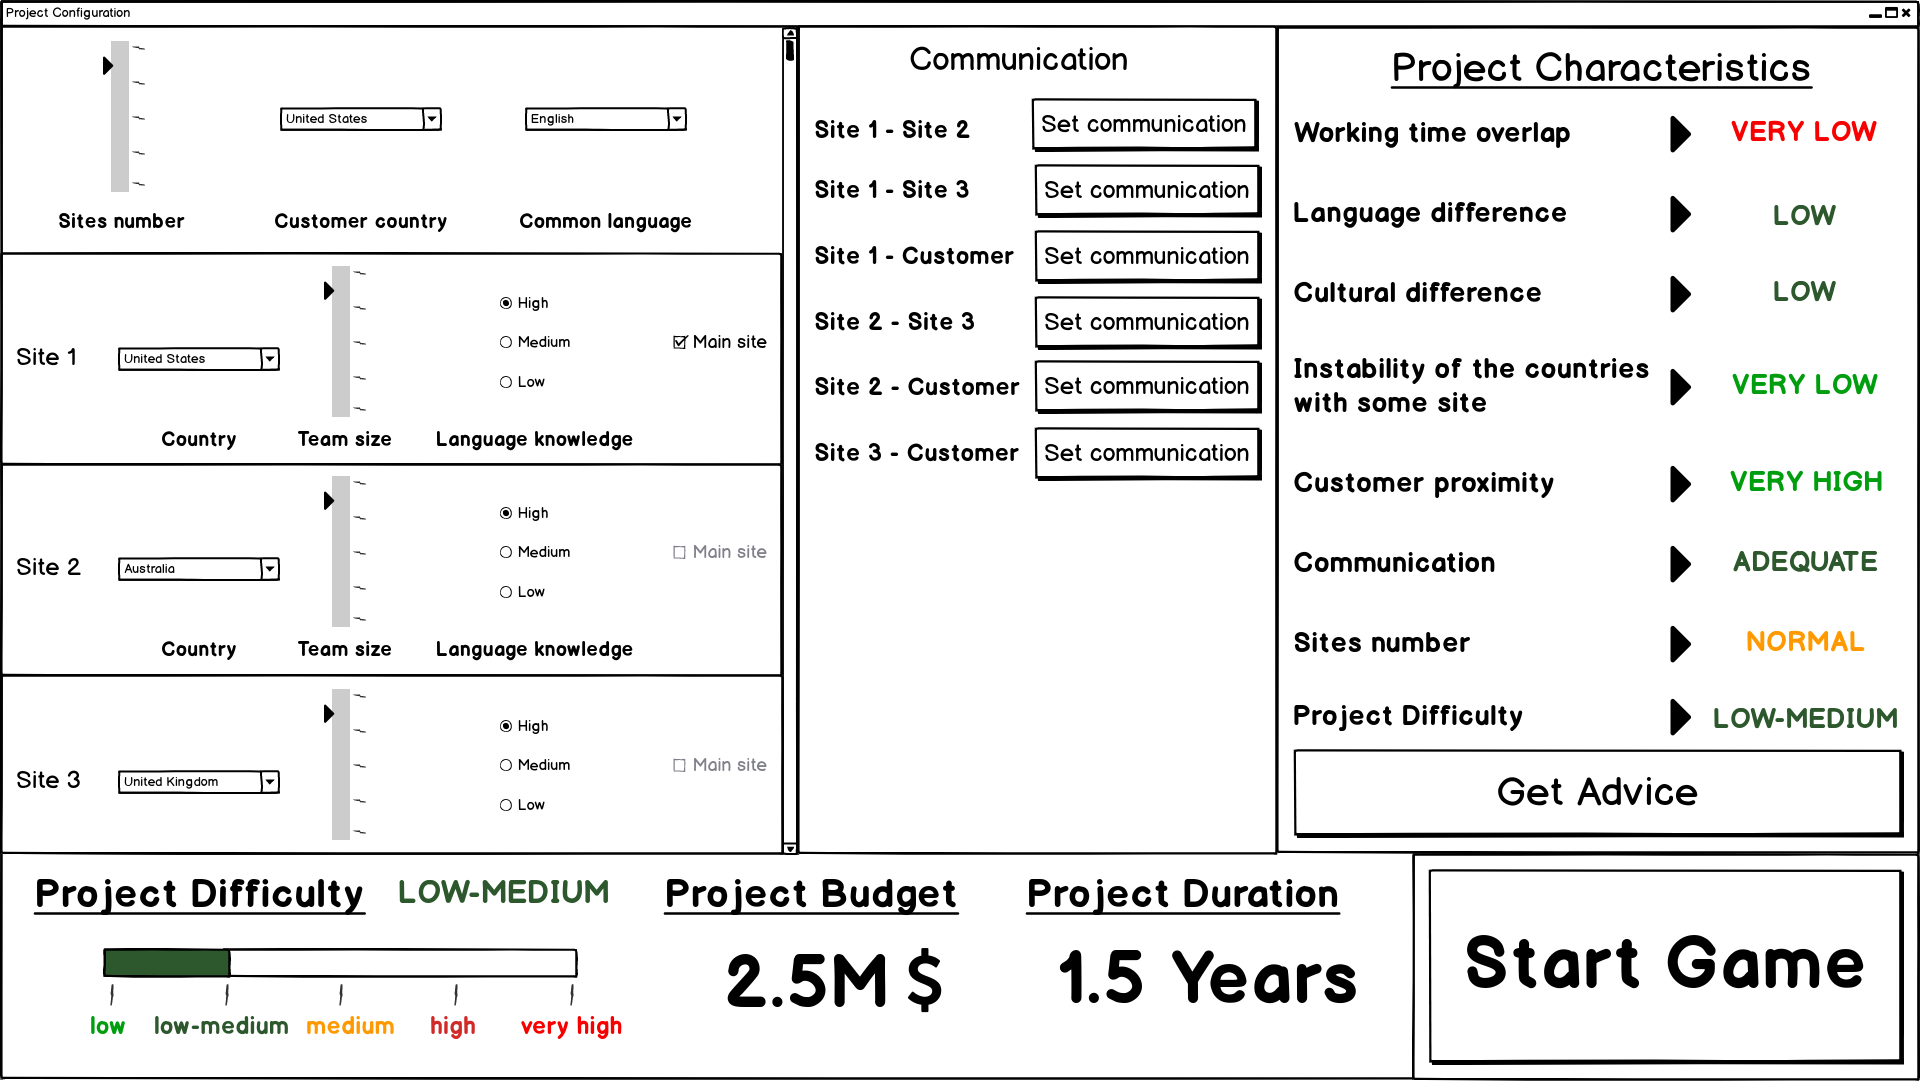
\includegraphics[width=1\linewidth]{VentanaConfiguracionBoceto}
	\caption[Boceto de la ventana de configuración del proyecto]{Boceto de la ventana de configuración del proyecto}
	\label{fig:VentanaConfiguracionBoceto}
\end{figure}

Como se puede observar, se ha optado por un diseño, en el cual, los elementos relacionados con la configuración del proyecto se mantengan en todo momento en pantalla, mientras el jugador interacciona con ellos. De esta manera, conseguimos que el jugador analice todos los elementos a configurar de un vistazo. Los parámetros que tienen que ser configurados están relacionados con conceptos básicos y componentes característicos de un proyecto de DGS, como pueden ser: el número de sites del proyecto, el país donde se ubica tanto el cliente como los demás equipos de trabajo, el número de trabajadores por cada equipo de trabajo, el idioma principal de comunicación entre los miembros del proyecto o la ubicación del site principal de desarrollo del proyecto. Por otro lado, el jugador también configurará las herramientas con las que se comunicarán cada uno de los equipos de trabajo del proyecto. Además, en la interfaz se mostrarán un conjunto de características referentes a un proyecto global y se indicará mediante el uso de etiquetas lingüísticas su valor en el proyecto configurado. Con ello, también se mostrará la dificultad de llevar a cabo la gestión del proyecto con dicha configuración. Cabe destacar, que se proporcionará un botón para obtener recomendaciones que nos indiquen que parámetros se deben cambiar para reducir la dificultad del proyecto, destinado a aquellos jugadores menos experimentados. Otra información relevante como la duración o el presupuesto inicial del proyecto también se presentan en esta interfaz.

Con este boceto, perseguimos que el jugador adquiera y se familiarice con los conceptos y elementos básicos de los proyectos DGS, aprenda como estos elementos modifican las características del proyecto y su dificultad, y conozca que configuraciones de proyectos son más fáciles de gestionar y cuales más complicadas.

\subsection{HDU02 - Boceto de la ventana de juego}
\label{sec:HDU02}

En segundo lugar, como segunda historia de usuario del presente sprint se procedió a diseñar el boceto de la interfaz de juego de Global-Manager, la segunda fase en la que se basará cada partida. Esta interfaz permitirá a los jugadores llevar a cabo la gestión de diferentes proyectos como jefes de proyecto.

Al igual que en el desarrollo del anterior boceto, se han evaluado diferentes juegos para comprobar como son sus fases de juego, para adaptar y mejorarlas en nuestro juego. Además, se ha vuelto a utilizar la herramienta para el diseño de bocetos \emph{Balsamiq Mockups}.

Una vez el jugador configura un proyecto, se procederá con la fase de juego. En esta parte de la partida, se lleva a cabo una simulación del proyecto DGS configurado. En la figura \ref{fig:VentanaJuegoBoceto}, se puede observar el boceto de la interfaz de juego.

\begin{figure}[htb]
	\centering
	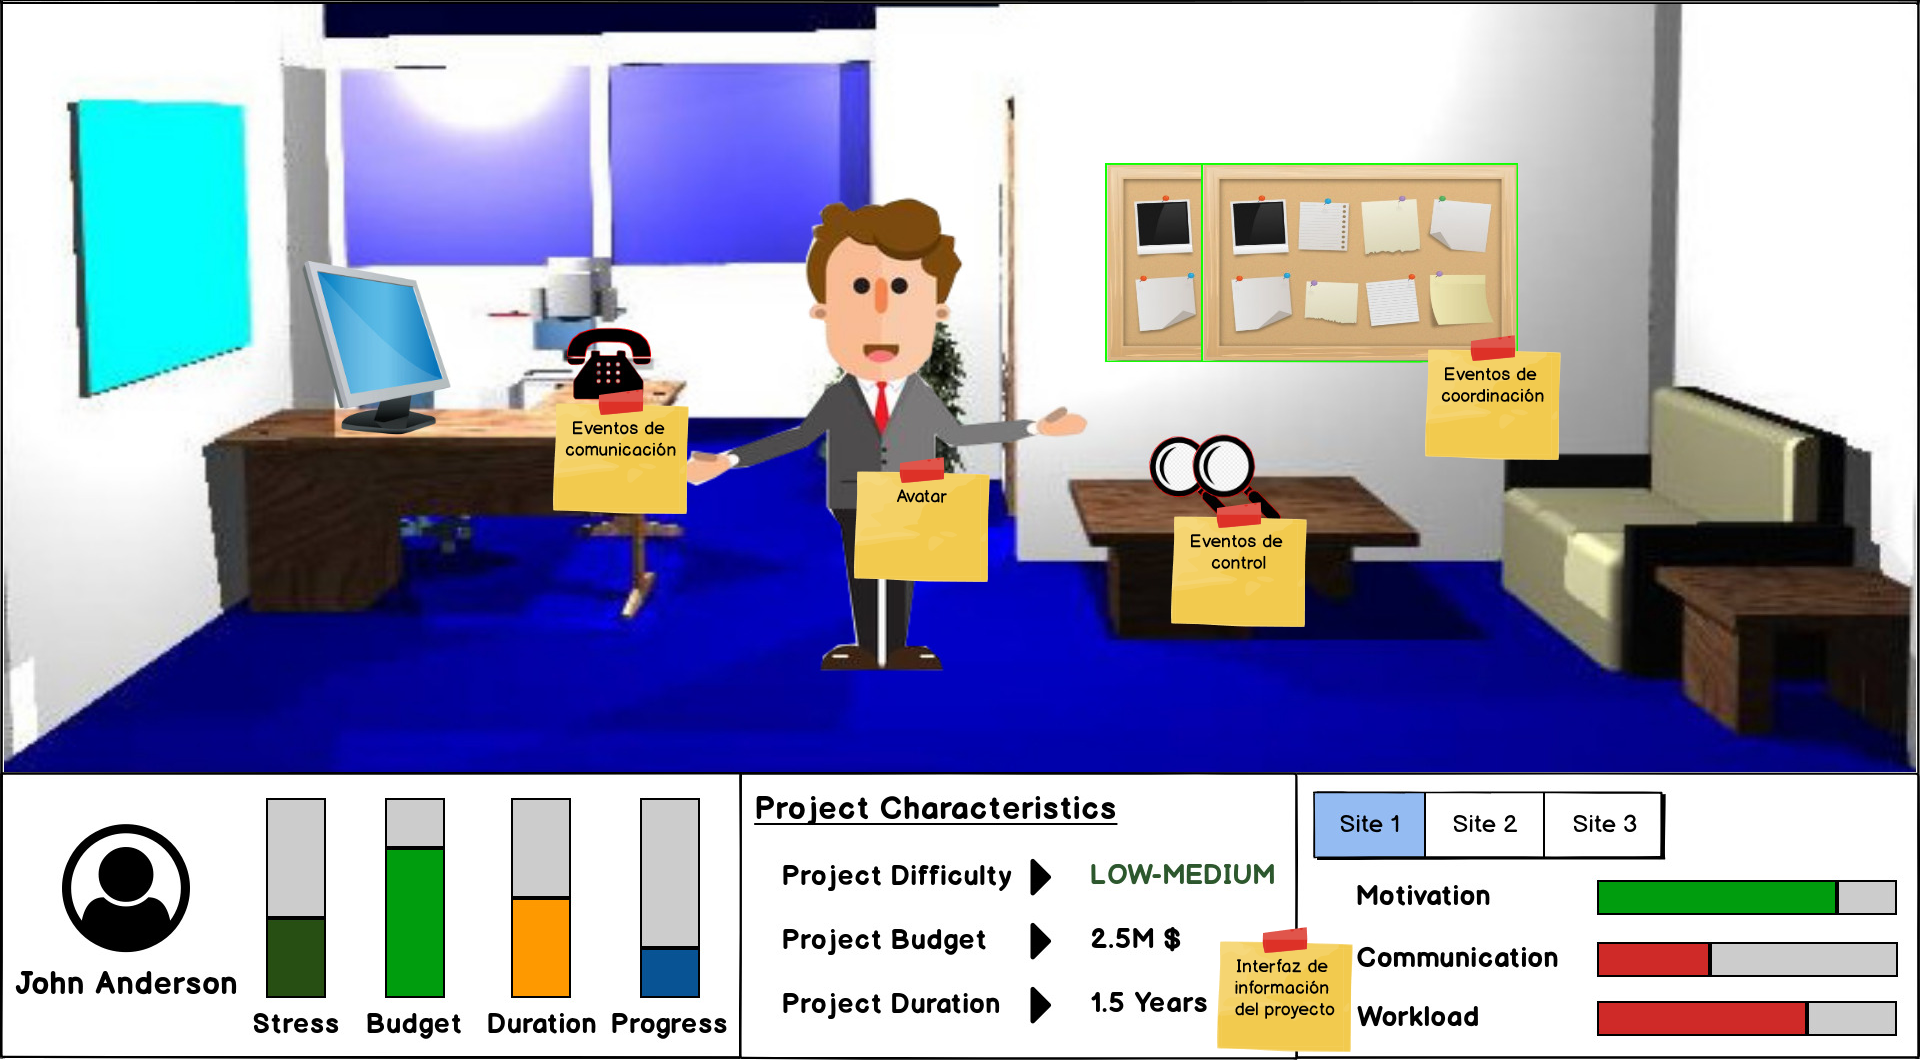
\includegraphics[width=1\linewidth]{VentanaJuegoBoceto}
	\caption[Boceto de la ventana de juego]{Boceto de la ventana de juego}
	\label{fig:VentanaJuegoBoceto}
\end{figure}

En esta ventana, aparecería el entorno de juego, el cual se correspondería con el de una oficina, junto con un avatar del personaje, el cual representaría al jugador. En este escenario, caerían diferentes objetos, los cuales representarían situaciones o eventos que pueden ocurrir en estos proyectos. Estos eventos podrán ser buenos, con una repercusión positiva en el proyecto o malos, en cuyo caso consistirían en impedimentos (representados a través de una pregunta) ocurridos en el proyecto y el jugador, en el rol de jefe de proyecto, deberá solventar dicha situación escogiendo la mejor opción (mejor respuesta entre varias). Estos eventos hacen referencia a los tres grandes desafíos de los proyectos DGS: teléfono (comunicación), post-it (coordinación) y lupa (control). Por otro lado, en la parte inferior de la ventana aparecería información relevante sobre el proyecto que se está gestionando, como el estrés del jugador, el presupuesto, la duración o el progreso actual del proyecto que se representaría a través de barras de progreso; información inicial como dificultad, presupuesto o duración inicial; e información sobre cada uno de los sites como motivación, comunicación con los demás sites o carga de trabajo, representado mediante barras de progreso.

De esta manera, buscamos que el jugador se sienta en la piel de un jefe de proyecto DGS y aprenda a hacer frente las dificultades que conlleva gestionar esta clase de proyectos, en especial los relacionados con la comunicación, coordinación y control.

\subsection{HDU07 - Diseñar la base de datos}
\label{sec:HDU07}

Tras haber realizado los bocetos de las interfaces más importantes de Global-Manager, es necesario la creación de una base de datos, la cual será utilizada por el juego para obtener datos relevantes y almacenar la información de las diferentes partidas. Para la creación de la base de datos, se ha optado por la utilización de \emph{SQLite} como motor de base de datos y la herramienta \emph{DB Browser (SQLite)} para la manipulación de los datos de dicha base de datos.

Esta base de datos debe permitir almacenar la información sobre las entidades que manipulará el juego. Estas son: los jugadores que juegan las partidas, las diferentes configuraciones que se realizan de los proyectos junto con la configuración de cada site del proyecto, y la evolución y resultado de las partidas.

Con todo esto en cuenta, se ha llevado a cabo el diseño de la siguiente base de datos, la cual puede observarse un esquema de su modelo relacional en la figura \ref{fig:ModeloRelacionalBBDD}.

\begin{figure}[htb]
	\centering
	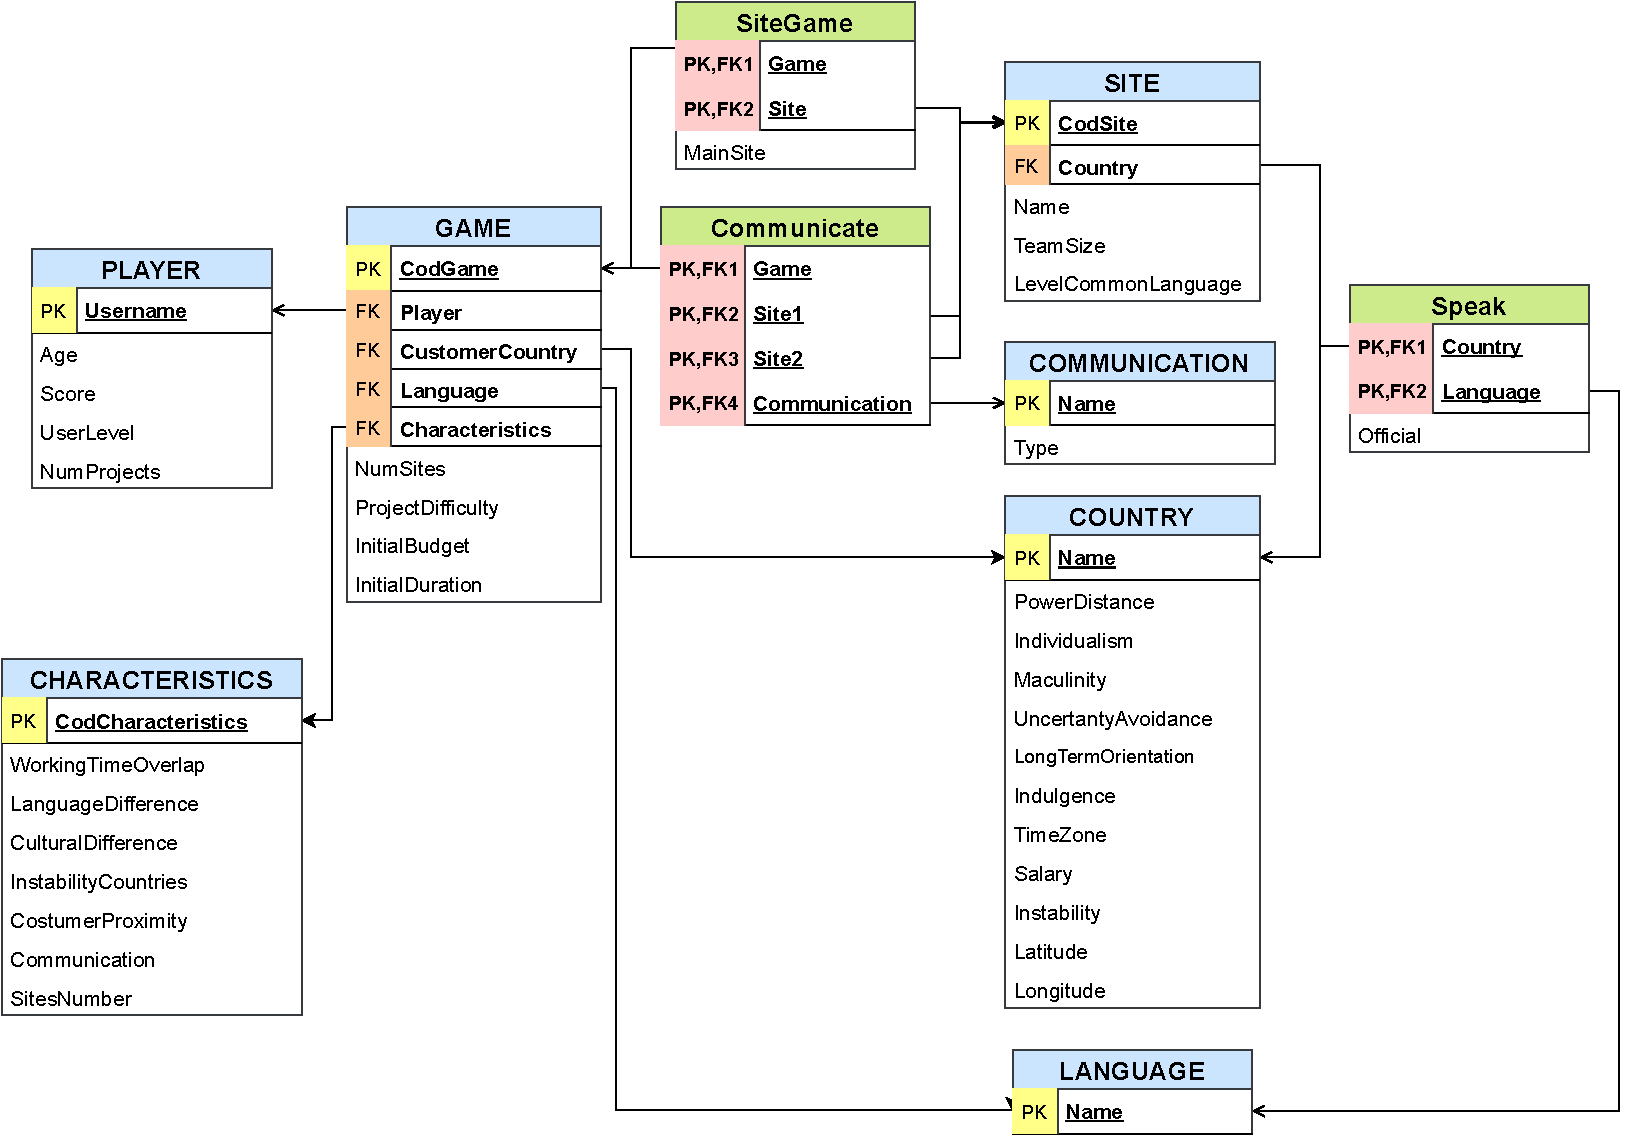
\includegraphics[width=1\linewidth]{ModeloRelacionalBBDD}
	\caption[Modelo relacional de la base de datos]{Modelo relacional de la base de datos}
	\label{fig:ModeloRelacionalBBDD}
\end{figure}

En primer lugar, se tiene la información relativa a los jugadores, la cual se almacena en la entidad \emph{PLAYER}, la cual tendrá asociado un nombre de usuario, la edad, una puntuación, el nivel de jugador actual y el número de proyectos (partidas) gestionados.

Como principal entidad se dispone la tabla \emph{GAME}, en la cual se almacena toda la información general de una partida (tanto de la evolución de la partida como de la configuración inicial del proyecto). Su información relevante es: el código del juego, el nombre del jugador, el nombre del país donde se encuentra el cliente, el idioma común, las características del proyecto, el número de sites, el nivel de dificultad y el presupuesto y duración inicial del proyecto.

Las características del proyecto que se almacenan en la base de datos (en la entidad \emph{CHARACTERISTICS}) son las que se mostraron anteriormente en el boceto de la ventana de configuración del proyecto, en la figura \ref{fig:VentanaConfiguracionBoceto}. Estas características son: el solapamiento del tiempo de trabajo, la diferencia lingüística, la distancia cultural, la existencia de países inestables en el proyecto, la proximidad al cliente, la comunicación y el número de sites.

Por otro lado, también se almacenarán las configuraciones de los diferentes sites de los proyectos, en la entidad \emph{SITE}. En esta tabla, se guardará un código numérico del site, el nombre del país donde se encuentra el site, el nombre asociado a dicho site, el tamaño del equipo de trabajo y el nivel de conocimiento del idioma común del proyecto. Dicha entidad estará vinculada con la tabla \emph{GAME} a través de la tabla N:M \emph{SiteGame}, para indicar que configuraciones de sites pertenecen a una determinada partida. Dicha tabla, también se utilizará para indicar que determinado site es el seleccionado para ser el principal del proyecto.

Como se ha indicado anteriormente, cada site y cada cliente se encontrará en un país determinado, por lo que es necesario tener registrada la información relevante de un conjunto de países. De cada país, se guardará su nombre en inglés, un conjunto de parámetros obtenidos a partir del \emph{Modelo de las 6 dimensiones de Hofstede}\footnote{Información del valor de las dimensiones de cada país obtenida mediante la página web \url{https://www.hofstede-insights.com/}} \cite{hofstede2011dimensionalizing} utilizados para identificar los comportamientos culturales de cada país, la zona horaria\footnote{\url{https://24timezones.com/reloj_hora_exacta.php\#/map}}, el salario medio de un ingeniero software en horas\footnote{\url{https://info.caprelo.com/blog/average-job-salaries-around-the-world}}, si el país se encuentra entre uno de los países inestables\footnote{\url{https://es.gizmodo.com/los-60-paises-mas-inestables-del-mundo-en-un-solo-mapa-559488437}} y su ubicación en el mundo con su latitud y longitud\footnote{\url{https://es.distance.to/}}. A continuación, en el código \ref{lst:InsertarPais} se muestra un ejemplo del comando SQL utilizado para añadir la información necesaria de cada país.

\lstinputlisting[style=SQL-color,float=ht,caption={Código SQL para insertar la información relevante del país España},label=lst:InsertarPais]{../scripts/InsertarPais.sql}

También es necesario almacenar los diferentes idiomas que se hablan en un determinado país o el idioma común con el que se comunicarán los miembros del proyecto. Para ello, se ha utilizado la entidad \emph{LANGUAGE} para registrar un conjunto de idiomas por su nombre en ingles. Además, con la tabla N:M \emph{Speak} son almacenados los idiomas que hablan los diferentes países registrados en la base de datos, indicando junto a ello si se trata de un idioma oficial en dicho país. En el código \ref{lst:InsertarSpeak} se muestra un ejemplo del comando SQL utilizado para añadir los idiomas que habla un determinado país.

\lstinputlisting[style=SQL-color,float=ht,caption={Código SQL para insertar los idiomas que se hablan en Argentina},label=lst:InsertarSpeak]{../scripts/InsertarSpeak.sql}

Por último, se almacenará en la base de datos la configuración que el jugador ha realizado sobre la comunicación del proyecto, es decir, que herramientas de comunicación utilizará cada site para comunicarse con el resto. Para ello, se utilizará la tabla N:M \emph{Communicate}, en la cual se guardará la herramienta de comunicación que utilizarán dos determinado site en una partida. El conjunto de herramientas de comunicación existentes en el juego se registrarán en la entidad \emph{COMMUNICATION} y en ella se indicará su tipo (si conlleva una comunicación sincronía o asíncrona). En el código \ref{lst:InsertarComunicacion} se muestra un ejemplo del comando SQL utilizado para añadir las herramientas de comunicación.

\lstinputlisting[style=SQL-color,float=ht,caption={Código SQL para insertar la información de la herramienta de comunicación teléfono},label=lst:InsertarComunicacion]{../scripts/InsertarComunicacion.sql}

Adicionalmente, serán necesarias nuevas vistas y modificaciones que serán desarrolladas en los sprints correspondientes.

\subsection{Revisión del Sprint}
\label{sec:RevisionSprint1}

En el presente sprint se han realizado las revisiones de los artefactos obtenidos, en primer lugar de los bocetos de configuración del proyecto y juego, y en segundo lugar de la base de datos diseñada. Tras finalizar dicha validación, se ha dado por finalizado el primer incremento del proyecto.

En primer lugar, los bocetos tuvieron una gran aceptación por parte del dueño del producto. El boceto de configuración del proyecto sufrió una ligera modificación, ya que el primer diseño de la fase de configuración de la comunicación iba a ser un conjunto de botones (tantos como combinaciones entre sites hubiera), y cada botón abriría una pequeña ventana donde el jugador podría seleccionar las herramientas de comunicación. Este diseño fue rechazado por el dueño del producto, ya que era demasiado confuso y se necesitaba que toda la información permaneciese en la misma ventana. Por ello, se optó por introducir dicha configuración directamente en la misma ventana mediante botones que representasen cada herramienta de comunicación. Además, en el primer diseño de la configuración de la comunicación se tenía en cuenta al cliente, sin embargo en el boceto final se suprimió.

\begin{figure}[htb]
	\centering
	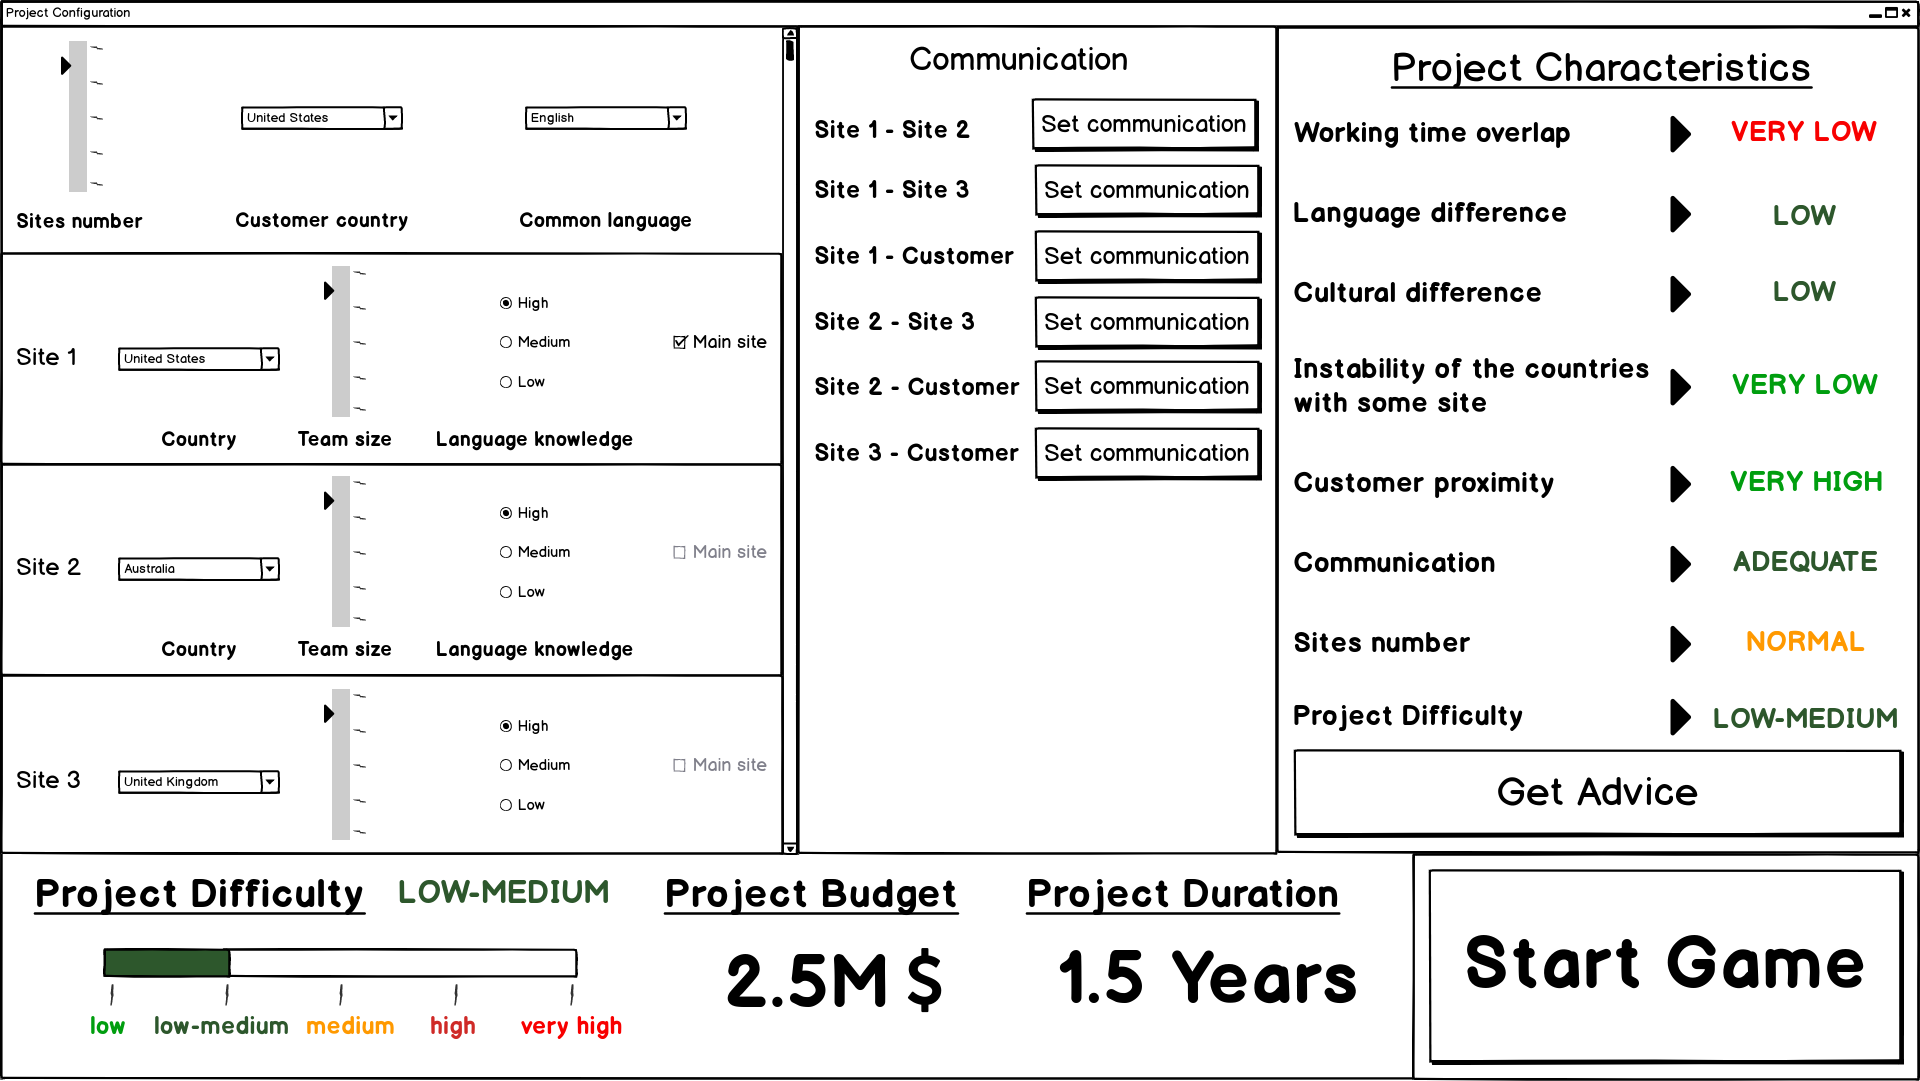
\includegraphics[width=1\linewidth]{VentanaConfiguracionBocetoInicial}
	\caption[Boceto inicial de la ventana de configuración del proyecto]{Boceto inicial de la ventana de configuración del proyecto}
	\label{fig:VentanaConfiguracionBocetoInicial}
\end{figure}

Por otro lado, el boceto de la ventana de juego no sufrió ningún cambio, ya que la idea inicial fue la que se mantuvo. 

Por último, la propuesta inicial de la base de datos también fue aceptada, pero cabe destacar que se realizaron algunas correcciones en los tipos y atributos que no supusieron un problema.

\subsection{Incidencias del Sprint}
\label{sec:IncidenciasSprint1}

Cabe destacar que el primer sprint del proyecto no ha resultado ser especialmente problemático:
\begin{itemize}
	\item Los bocetos iniciales del juego desarrollados durante el sprint fueron aceptados prácticamente en su totalidad, salvo a excepción de algunas modificaciones en la ventana de configuración del proyecto como se indicó en la subsección anterior.
	\item En un primer lugar, el diseño de la base de datos fue aceptado sin problemas, sin embargo en los posteriores sprint se tuvieron que llevar a cabo algunas modificaciones.
	\item Cabe destacar, que fue necesario conocer el sistema de gestión de base de datos \emph{SQLite}, sin embargo al ser relacional y parecido al motor \emph{MySQL}, aprendido a lo largo de la carrera no supuso problema alguno.
\end{itemize}

\newpage

\section{Sprint 2}
\label{sec:Sprint2}

El presente sprint dará comienzo el desarrollo de Global-Manager con el diseño de las interfaces gráficas de la ventana de cuestionario de nivel para la creación de un nuevo jugador, en primer lugar, y con la ventana de configuración del proyecto en segundo lugar, utilizando como base el boceto desarrollado en la historia de usuario 1 (véase sección \ref{sec:HDU01}). 

\subsection{Planificación del Sprint}
\label{sec:PlanificacionSprint2}

A continuación, se detalla toda la información de cada historia de usuario de la pila del presente sprint. Este sprint esta compuesto por dos historias de usuario, como se describió en la sección \ref{sec:PlanificacionProyecto}, las cuales son las siguientes:

\begin{table}[htb]
\centering
\arrayrulecolor{white}
\resizebox{\textwidth}{!}{%
\begin{tabular}{ccc}
\rowcolor[HTML]{EB6D0B} 
\multicolumn{1}{c|}{\cellcolor[HTML]{EB6D0B}{\color[HTML]{FFFFFF} Sprint 2}} &
  \multicolumn{1}{c|}{\cellcolor[HTML]{EB6D0B}{\color[HTML]{FFFFFF} HDU03}} &
  \cellcolor[HTML]{F5D2A8}{\color[HTML]{333333} Diseñar la ventana cuestionario de nivel} \\ \hline
\rowcolor[HTML]{EB6D0B} 
\multicolumn{3}{c}{\cellcolor[HTML]{EB6D0B}{\color[HTML]{FFFFFF} Descripción}} \\ \hline
\rowcolor[HTML]{F5D2A8} 
\multicolumn{3}{l}{\cellcolor[HTML]{F5D2A8}\begin{tabular}[c]{@{}l@{}}Quiero una interfaz gráfica en donde un jugador que no ha jugado nunca, pueda crearse un nuevo perfil de \\ jugador introduciendo datos relacionados como un nombre de usuario o la edad. Deberá existir también un \\ pequeño cuestinario para conocer los conocimientos en DGS y gestión de proyectos del jugador.\end{tabular}} \\ \hline
\rowcolor[HTML]{EB6D0B} 
\multicolumn{3}{c}{\cellcolor[HTML]{EB6D0B}{\color[HTML]{FFFFFF} Resumen de las tareas}} \\ \hline
\rowcolor[HTML]{F5D2A8} 
\multicolumn{3}{l}{\cellcolor[HTML]{F5D2A8}\begin{tabular}[c]{@{}l@{}}- Diseñar interfaz gráfica\\  - Realizar entrevista a un experto para conocer como extraer los conocimientos en DGS y gestión de \\  proyectos que tenga una persona\\  - Crear cuestionario de nivel\\  - Introducir cuestionario de nivel en la interfaz gráfica\\  - Presentar resultados al dueño del producto - Modificar los cambios propuestos\end{tabular}} \\ \hline
\rowcolor[HTML]{EB6D0B} 
\multicolumn{1}{c|}{\cellcolor[HTML]{EB6D0B}{\color[HTML]{FFFFFF} Estimación}} &
  \multicolumn{1}{c|}{\cellcolor[HTML]{EB6D0B}{\color[HTML]{FFFFFF} Valor (1/10)}} &
  {\color[HTML]{FFFFFF} Dependencias} \\ \hline
\rowcolor[HTML]{F5D2A8} 
\multicolumn{1}{c|}{\cellcolor[HTML]{F5D2A8}6 días} &
  \multicolumn{1}{c|}{\cellcolor[HTML]{F5D2A8}7} &
  -
\end{tabular}%
}
\caption{Historia de usuario 3: Diseñar la ventana cuestionario de nivel}
\label{tab:HDU03}
\end{table}

\begin{table}[htb]
\centering
\arrayrulecolor{white}
\resizebox{\textwidth}{!}{%
\begin{tabular}{ccc}
\rowcolor[HTML]{EB6D0B} 
\multicolumn{1}{c|}{\cellcolor[HTML]{EB6D0B}{\color[HTML]{FFFFFF} Sprint 2}} &
  \multicolumn{1}{c|}{\cellcolor[HTML]{EB6D0B}{\color[HTML]{FFFFFF} HDU04}} &
  \cellcolor[HTML]{F5D2A8}{\color[HTML]{333333} Diseñar la ventana de configuración del proyecto} \\ \hline
\rowcolor[HTML]{EB6D0B} 
\multicolumn{3}{c}{\cellcolor[HTML]{EB6D0B}{\color[HTML]{FFFFFF} Descripción}} \\ \hline
\rowcolor[HTML]{F5D2A8} 
\multicolumn{3}{l}{\cellcolor[HTML]{F5D2A8}\begin{tabular}[c]{@{}l@{}}Quiero una interfaz gráfica en donde el jugador pueda configurar un proyecto DGS desde cero y pueda \\ visualizar diferentes conceptos relacionados con DGS y parámetros necesarios a configurar\end{tabular}} \\ \hline
\rowcolor[HTML]{EB6D0B} 
\multicolumn{3}{c}{\cellcolor[HTML]{EB6D0B}{\color[HTML]{FFFFFF} Resumen de las tareas}} \\ \hline
\rowcolor[HTML]{F5D2A8} 
\multicolumn{3}{l}{\cellcolor[HTML]{F5D2A8}\begin{tabular}[c]{@{}l@{}}- Diseñar configuración inicial del proyecto\\  - Diseñar la configuración de cada site\\  - Diseñar la configuración de la comunicación entre sites\\  - Diseñar la visualización de las características del proyecto\\  - Diseñar la visualización de la dificultad del proyecto\\  - Presentar resultados al dueño del producto\\  - Modificar los cambios propuestos\end{tabular}} \\ \hline
\rowcolor[HTML]{EB6D0B} 
\multicolumn{1}{c|}{\cellcolor[HTML]{EB6D0B}{\color[HTML]{FFFFFF} Estimación}} &
  \multicolumn{1}{c|}{\cellcolor[HTML]{EB6D0B}{\color[HTML]{FFFFFF} Valor (1/10)}} &
  {\color[HTML]{FFFFFF} Dependencias} \\ \hline
\rowcolor[HTML]{F5D2A8} 
\multicolumn{1}{c|}{\cellcolor[HTML]{F5D2A8}8 días} &
  \multicolumn{1}{c|}{\cellcolor[HTML]{F5D2A8}8} &
  HDU01
\end{tabular}%
}
\caption{Historia de usuario 4: Diseñar la ventana de configuración del proyecto}
\label{tab:HDU04}
\end{table}

Tras la finalización del segundo sprint se conseguirán como resultado los siguientes artefactos:
\begin{itemize}
	\item Prototipo de la interfaz de cuestionario de nivel
	\item Prototipo de la interfaz para la configuración del proyecto
\end{itemize}

\subsection{HDU03 - Diseñar la ventana cuestionario de nivel}
\label{sec:HDU03}

En primer lugar, para iniciar la creación del juego, se ha comenzado con el desarrollo del diseño de una interfaz con la cual el jugador, si no posee ningún perfil almacenado en el juego, pueda crearse uno nuevo. A través de este perfil de jugador, se podrá llevar a cabo un seguimiento de las partidas realizadas y evaluar como evoluciona su flujo de aprendizaje. Por otro lado, mediante esta interfaz se pretende calcular los conocimientos actuales del jugador sobre DGS y gestión de proyectos y obtener de esta manera un nivel de jugador que nos indique el grado de conocimiento. Para llevar a cabo dicho cálculo, se utilizará un cuestionario con diferentes preguntas sobre la experiencia del jugador, conocimiento que posea y conceptos básicos de DGS y gestión de proyectos. De esta manera, el jugador rellenará el cuestionario con el objetivo de crear un perfil, pero también se evaluarán sus conocimientos para obtener un nivel de jugador y ofrecer una experiencia de usuario acorde a sus conocimientos. 

Para componer el cuestionario para el cálculo del nivel de jugador, nos apoyamos en una pequeña entrevista realizada a la experta en DGS y co-tutora de este TFG, Aurora Vizcaíno Barceló, con el objetivo de conocer cuales son las componentes que se deben tener en cuenta para extraer el grado de conocimiento de una persona en dicho tema. Además de las preguntas extraídas de la entrevista, se añadieron algunas más, variación de las ya obtenidas. A continuación en la figura \ref{fig:VentanaCuestionarioNivel}, se muestra el resultado final de la interfaz gráfica de la ventana cuestionario de nivel, con el conjunto de preguntas seleccionadas.

\begin{figure}[htb]
	\centering
	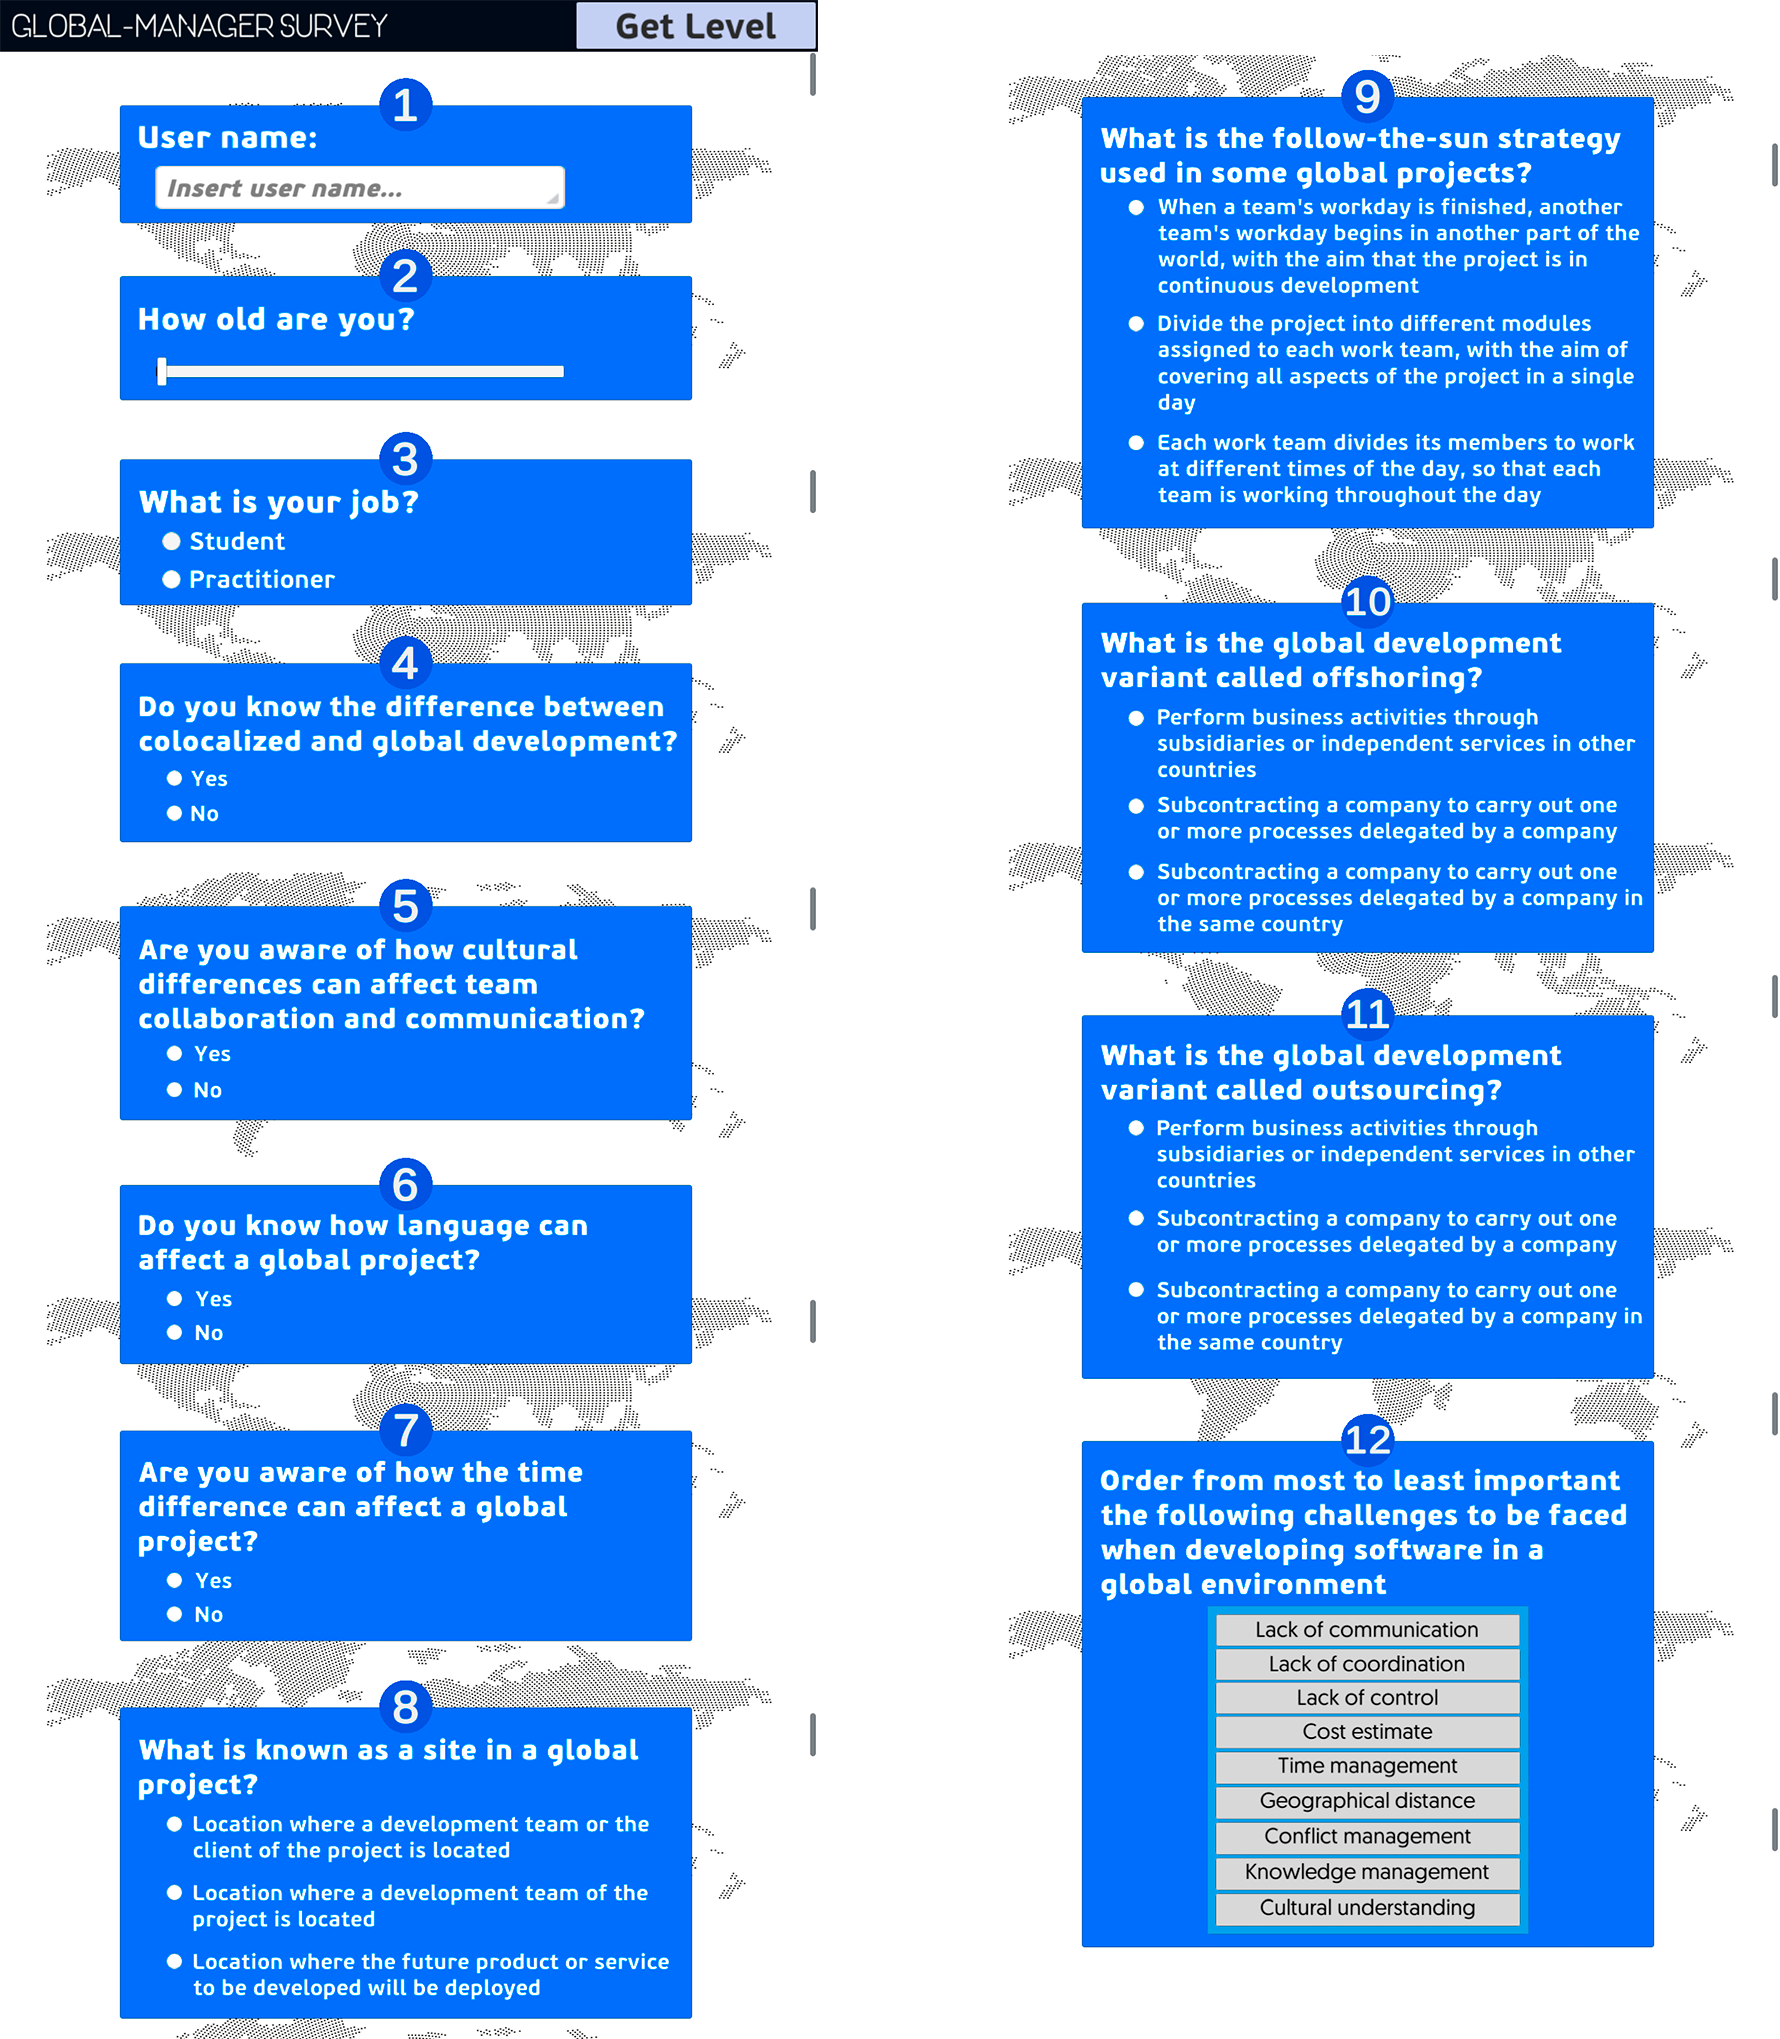
\includegraphics[width=1\linewidth]{VentanaCuestionarioNivel}
	\caption[Ventana del cuestionario de nivel]{Ventana del cuestionario de nivel}
	\label{fig:VentanaCuestionarioNivel}
\end{figure}

Como se puede observar, el cuestionario consta de un total de doce cuestiones generales, donde la mayoría de ellas se corresponden con preguntas tipo test. Las dos primeras preguntas aluden a información relevante del jugador, como es el nombre de usuario que se desea tener y la edad que posee. Seguidamente, se encontrarán un total de nueve preguntas tipo test, las cuales podemos dividir en tres grandes grupos:

\begin{itemize}
	\item \textbf{Pregunta 3:} Se corresponde con una pregunta utilizada para conocer la situación actual del jugador, es decir, si se encuentra estudiando o trabajando profesionalmente en el mercado, dependiendo de la respuesta, se realizarán al final del cuestionario una clase de preguntas diferentes. En el caso de que la respuesta sea estudiante (\emph{Student}), se mostrarán las preguntas de la figura \ref{fig:PreguntasStudent}, de igual manera, si la respuesta fuese profesional (\emph{Practitioner}), las preguntas mostradas serían las de la figura \ref{fig:PreguntasPractitioner}.
	\item \textbf{Preguntas 4-7:} Consisten en un conjunto de cuestiones tipo test donde las respuestas son: sí poseo los conocimientos (\emph{Yes}), y no poseo los conocimientos (\emph{No}). Estas cuestiones sirven para conocer los conocimientos actuales que posee el jugador del tema de DGS y gestión de proyectos en relación con \emph{diferencia entre desarrollo colocalizado y global}, \emph{diferencia cultural}, \emph{desigualdad lingüística} y \emph{disparidad horaria} en un proyecto global.
	\item \textbf{Preguntas 8-11:} Se corresponden con un conjunto de preguntas tipo test sobre elementos y conceptos básicos sobre la gestión en proyectos de software globales. Estas preguntas hacen referencia a los conceptos de: \emph{site}, \emph{estrategia follow-the-sun}, \emph{offshoring} y \emph{outsourcing}. A continuación, se muestra una traducción de cada pregunta junto con su respuesta correcta:
	\begin{itemize}
		\item \textbf{¿Qué es lo que se conoce como un site en un proyecto global?} Ubicación donde se encuentra un equipo de desarrollo del proyecto.
		\item \textbf{¿Qué es la estrategia follow-the-sun utilizada en algunos proyectos globales?} Cuando un equipo de trabajo acaba su jornada laboral, la jornada de otro equipo comienza en otra parte del mundo, con el objetivo de que el proyecto este en constante desarrollo.
		\item \textbf{¿Qué es la variante de desarrollo global llamada offshoring?} Realizar actividades de negocio a través de filiares o servicios independientes en otros países.
		\item \textbf{¿Qué es la variante de desarrollo global llamada outsourcing?} Subcontratar una compañía para llevar a cabo uno o más procesos delegados por la compañía.
	\end{itemize}
\end{itemize}

Prosiguiendo, en la siguiente cuestión (pregunta 12), se le pide al jugador que ordene de más a menos importante un conjunto de desafíos, que se pueden encontrar en entornos DGS. El orden correcto de la respuesta a esta pregunta, según el estudio realizado en \cite{niazi2016challenges} y la tabla \ref{tab:DificultadesDGS}, donde se citan los desafíos más importantes en los proyectos DGS, sería: \emph{cultural understanding}, \emph{lack of communication}, \emph{knowledge management}, \emph{time management}, \emph{lack of coordination}, \emph{lack of control}, \emph{conflict management}, \emph{cost estimate} y \emph{geographical distance}.

Por último, en función de la respuesta indicada del jugador en la pregunta 3, se mostrarán dos preguntas adicionales de tipo test con respuestas de \emph{Yes} y \emph{No}. En el caso de indicar el jugador que es estudiante, se mostrarán las preguntas de la figura \ref{fig:PreguntasStudent}, para conocer si ha estudiado DGS o gestión de proyectos. En caso contrario, si el jugador ha indicado que es profesional, se indicarán las preguntas de la figura \ref{fig:PreguntasPractitioner}, para conocer si alguna vez ha trabajado en un proyecto global o como jefe de proyecto.

\begin{figure}[htb]
	\centering
	\begin{subfigure}[b]{1\linewidth}
		\centering
		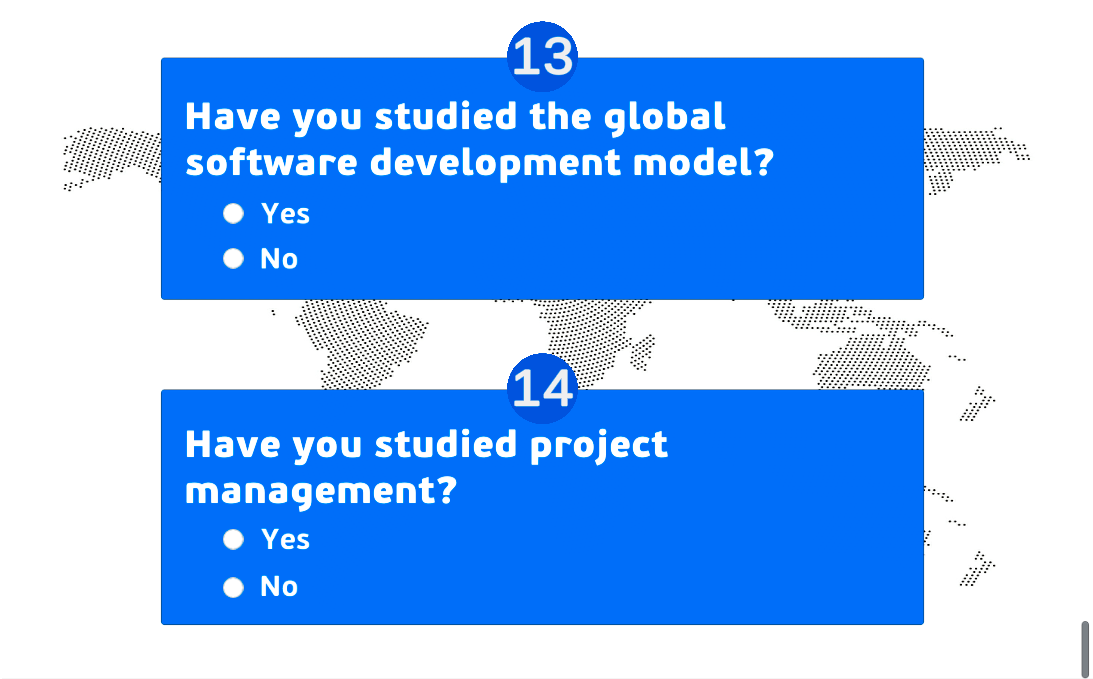
\includegraphics[width=0.8\linewidth]{PreguntasStudent}
		\caption{Preguntas para los estudiantes}\label{fig:PreguntasStudent}
	\end{subfigure}
	\begin{subfigure}[b]{1\linewidth}
		\centering
		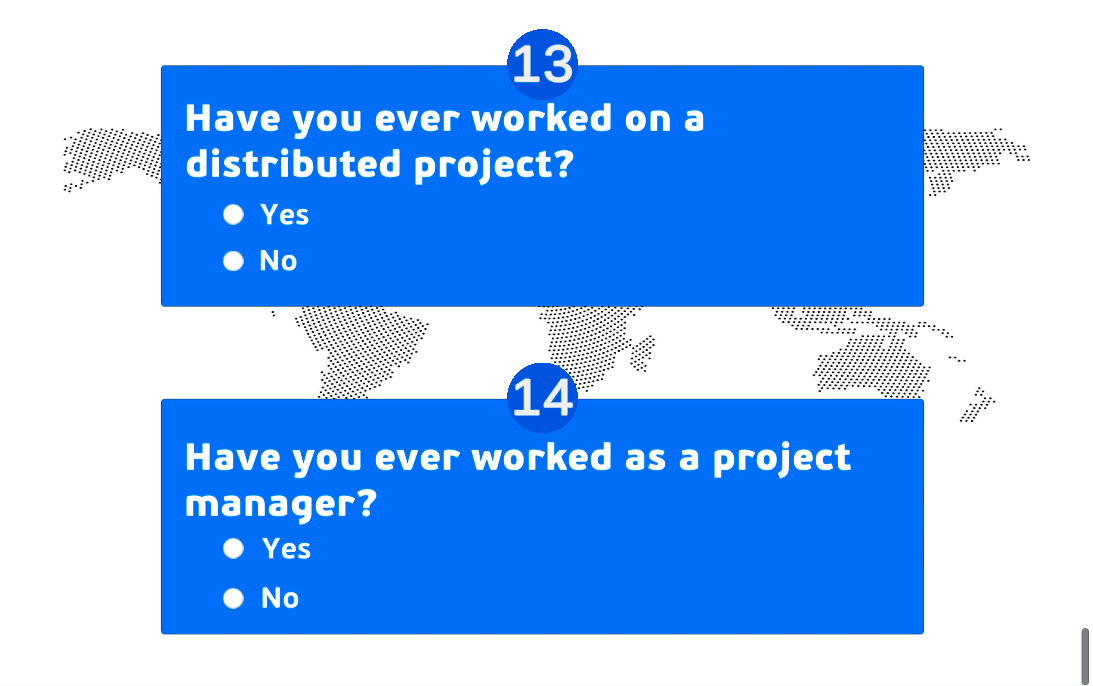
\includegraphics[width=0.8\linewidth]{PreguntasPractitioner}
		\caption{Preguntas para los profesionales}\label{fig:PreguntasPractitioner}
	\end{subfigure}
	\caption[Preguntas especializadas para estudiantes y profesionales]{Preguntas especializadas para estudiantes y profesionales}
	\label{fig:PreguntasAdicionales}
\end{figure}

\subsection{HDU04 - Diseñar la ventana de configuración del proyecto}
\label{sec:HDU04}

Una vez se ha desarrollado el diseño para la ventana cuestionario de nivel, donde se muestra un pequeño cuestionario con el cual el jugador puede crear y almacenar un nuevo usuario, y obtener un nivel de jugador acorde a sus conocimientos en el tema; es necesario comenzar a desarrollar la ejecución de las partidas. Para ello comenzaremos con el desarrollo del diseño de la intefaz de configuración del proyecto, permitiendo al jugador interactuar con diferentes elementos relacionados con la configuración de un proyecto de software global.

El diseño de la interfaz gráfica de la ventana de configuración del proyecto se puede observar en la siguiente figura \ref{fig:ConfigurationWindow}. La disposición del diseño de la ventana se puede dividir en siete partes diferentes: \emph{configuración inicial}, \emph{configuración de sites}, \emph{configuración de la comunicación}, \emph{características del proyecto}, \emph{presupuesto y duración}, \emph{dificultad del proyecto}, \emph{botón de empezar partida}.

\begin{figure}[htb]
	\centering
	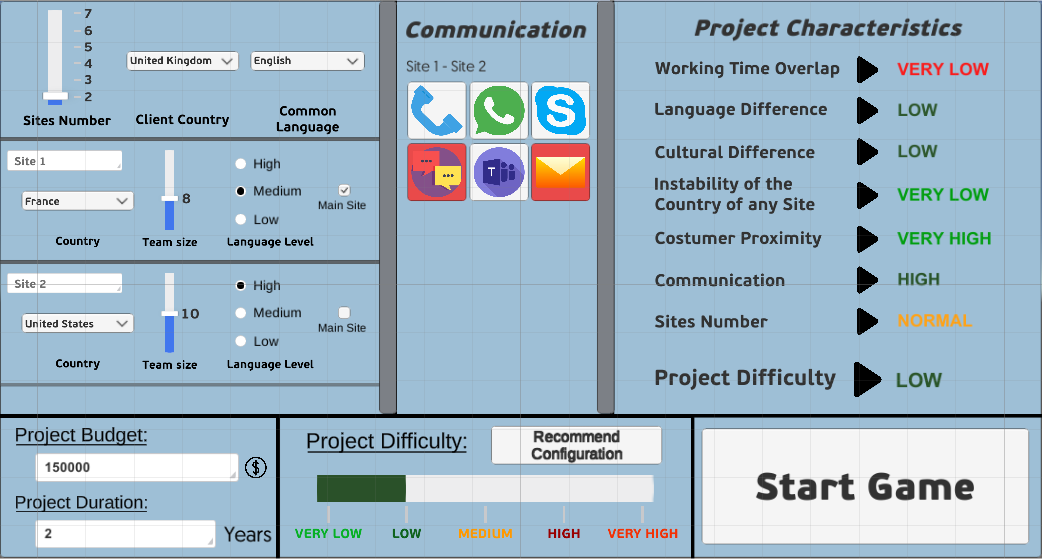
\includegraphics[width=1\linewidth]{ConfigurationWindow}
	\caption[Diseño de la ventana de configuración de un proyecto global]{Ventana de configuración del proyecto}
	\label{fig:ConfigurationWindow}
\end{figure}

A continuación, se indicará una pequeña descripción de cada una de las partes de la ventana de configuración del proyecto:

\begin{itemize}
	\item \textbf{Configuración inicial:} Corresponde a los primeros parámetros que el jugador debe de configurar, estos son: el número de sites (2-7) que compondrá el proyecto (mediante un slider), el país donde se encuentra el cliente (mediante un combo box) y el idioma con el que se comunicarán los diferentes miembros del proyecto (mediante un combo box).
	\item \textbf{Configuración de sites:} En función del número de sites definido anteriormente, se mostrará un cuadrado por cada site. El jugador deberá establecer los diferentes parámetros necesarios para cada site. Estos parámetros son: un nombre que lo distinga de los demás (mediante un campo de entrada), el país donde se encuentra el site (mediante un combo box), el tamaño del equipo de trabajo (2-20 miembros), el nivel del idioma definido anteriormente como idioma global del proyecto (se muestra mediante tres botones las opciones, \emph{high}, \emph{medium} y \emph{low}) y por último, el jugador indicará mediante el botón correspondiente a dicho site, aquel que se corresponda con el site central del proyecto.
	\item \textbf{Configuración de la comunicación:} Con el número de sites definido anteriormente, se mostrarán todas las combinaciones posibles entre los diferentes sites y el jugador tendrá que seleccionar mediante botones aquellas herramientas de comunicación que se utilizarán para llevar a cabo el intercambio de información en cada una de las combinaciones. Las herramientas de comunicación son las siguientes: \emph{teléfono}, \emph{WhatsApp}, \emph{Skype}, \emph{foros}, \emph{Microsoft Teams} y \emph{e-mail}.
	\item \textbf{Características del proyecto:} Se muestran un conjunto de características del proyecto o factores de éxito junto con la dificultad del proyecto. Estas características son recalculadas automáticamente en tiempo real en función de la configuración del proyecto actual realizada por el jugador. Estas caracteristicas poseen unas etiquetas lingüísticas para darles valor, estas son: \emph{VERY LOW}, \emph{LOW}, \emph{NORMAL}, \emph{HIGH} y \emph{VERY HIGH}. Estas características se han obtenido a partir del artículo \cite{vizcaino2013applying}, donde se ofrecen un conjunto de factores de éxito característicos en proyectos de desarrollo global, de estos se han seleccionado aquellos que resultan ser más fáciles de medir e implementar. Estas características son siete: solapamiento del tiempo de trabajo, diferencia lingüística, diferencia cultural, inestabilidad en algún país de alguno de los sites, proximidad al cliente, comunicación y número de sites.
	\item \textbf{Presupuesto y duración:} Mediante campos de entrada, el jugador deberá introducir dos valores reales, uno para indicar el presupuesto inicial del proyecto en dólares y otro para la duración inicial del proyecto en años.
	\item \textbf{Dificultad del proyecto:} El sistema calcula automáticamente en tiempo real la dificultad del proyecto en función de la configuración del proyecto que el jugador está llevando a cabo. Para mostrar dicha información visualmente, se ha utilizado una barra de progreso de 5 valores con etiquetas lingüísticas, de más fácil a más difícil, \emph{VERY LOW}, \emph{LOW}, \emph{MEDIUM}, \emph{HIGH} y \emph{VERY HIGH}. Se proporciona también un botón (Recommend Configuration), el cual se utilizará para ofrecer una configuración automática en función del nivel de jugador.
	\item \textbf{Botón de empezar partida:} Botón para comenzar la fase de juego con la simulación del proyecto.
\end{itemize}

\subsection{Revisión del Sprint}
\label{sec:RevisionSprin2}

En este segundo sprint se han revisado los diseños de los prototipos realizados para la interfaz de cuestionario de nivel y configuración del proyecto. Los dueños del producto los han aceptado en su totalidad salvo un pequeño cambio en la ventana de configuración del proyecto, ya que en el boceto inicial se diseñó un botón \emph{Recommendation}, el cual ofrecería consejos para reconfigurar el proyecto y reducir el nivel de dificultad, sin embargo, se ha modificado dicho botón por \emph{Recommend Configuration}, el cual deberá ofrecer una configuración aleatoria pero acorde con el nivel del jugador. De esta manera, se permite al jugador la oportunidad de que si no desea configurar un proyecto o no conoce los conocimientos necesarios para hacerlo, se le ofrezca uno automáticamente acorde con su aprendizaje.

\subsection{Incidencias del Sprint}
\label{sec:IncidenciasSprint2}

En el presente sprint, una de las incidencias más notables y que implicó algunos retrasos fue derivada del desconocimiento total de utilizar la plataforma de desarrollo de videojuegos, Unity:
\begin{itemize}
	\item Los diseños de las interfaces desarrollados durante el presente sprint fueron, en gran parte aceptados, salvo alguna modificación en la ventana de configuración del proyecto como se ha indicado anteriormente.
	\item La realización del presente sprint supuso manejar la plataforma de creación de videojuegos, Unity, por lo que en paralelo al desarrollo del sprint, se tuvo que aprender a manipular dicha herramienta ya que se tenía total desconocimiento. Para ello, se realizó un curso de Domestika\footnote{\url{https://www.domestika.org/es}} para obtener los conocimientos necesarios para crear videojuegos en 3D desde cero a través de la plataforma Unity.
\end{itemize}